%!TEX root = ../blob1.tex

\def\xxpar#1#2{\smallskip\noindent{\bf #1} {\it #2} \smallskip}
\def\mmpar#1#2#3{\smallskip\noindent{\bf #1} (#2). {\it #3} \smallskip}

\section{\texorpdfstring{$n$}{n}-categories and their modules}
\label{sec:ncats}

\subsection{Definition of \texorpdfstring{$n$}{n}-categories}
\label{ss:n-cat-def}

Before proceeding, we need more appropriate definitions of $n$-categories, 
$A_\infty$ $n$-categories, as well as modules for these, and tensor products of these modules.
(As is the case throughout this paper, by ``$n$-category" we mean some notion of
a ``weak" $n$-category with ``strong duality".)

Compared to other definitions in the literature,
the definitions presented below tie the categories more closely to the topology
and avoid combinatorial questions about, for example, finding a minimal sufficient
collection of generalized associativity axioms; we prefer maximal sets of axioms to minimal sets.
It is easy to show that examples of topological origin
(e.g.\ categories whose morphisms are maps into spaces or decorated balls, or bordism categories), 
satisfy our axioms.
To show that examples of a more purely algebraic origin satisfy our axioms, 
one would typically need the combinatorial
results that we have avoided here.

See \S\ref{n-cat-names} for a discussion of $n$-category terminology.

%\nn{Say something explicit about Lurie's work here? 
%It seems like this was something that Dan Freed wanted explaining when we talked to him in Aspen}

\medskip

The axioms for an $n$-category are spread throughout this section.
Collecting these together, an $n$-category is a gadget satisfying Axioms \ref{axiom:morphisms}, 
\ref{nca-boundary}, \ref{axiom:composition},  \ref{nca-assoc}, \ref{axiom:product}, \ref{axiom:extended-isotopies} and  \ref{axiom:splittings}.
For an enriched $n$-category we add Axiom \ref{axiom:enriched}.
For an $A_\infty$ $n$-category, we replace 
Axiom \ref{axiom:extended-isotopies} with Axiom \ref{axiom:families}.

Strictly speaking, before we can state the axioms for $k$-morphisms we need all the axioms 
for $k{-}1$-morphisms.
Readers who prefer things to be presented in a strictly logical order should read this 
subsection $n+1$ times, first setting $k=0$, then $k=1$, and so on until they reach $k=n$.

\medskip

There are many existing definitions of $n$-categories, with various intended uses.
In any such definition, there are sets of $k$-morphisms for each $0 \leq k \leq n$.
Generally, these sets are indexed by instances of a certain typical shape. 
Some $n$-category definitions model $k$-morphisms on the standard bihedron (interval, bigon, and so on).
Other definitions have a separate set of 1-morphisms for each interval $[0,l] \sub \r$, 
a separate set of 2-morphisms for each rectangle $[0,l_1]\times [0,l_2] \sub \r^2$,
and so on.
(This allows for strict associativity; see \cite{ulrike-tillmann-2008,0909.2212}.)
Still other definitions (see, for example, \cite{MR2094071})
model the $k$-morphisms on more complicated combinatorial polyhedra.

For our definition, we will allow our $k$-morphisms to have any shape, so long as it is 
homeomorphic to the standard $k$-ball.
Thus we associate a set of $k$-morphisms $\cC_k(X)$ to any $k$-manifold $X$ homeomorphic 
to the standard $k$-ball.
By ``a $k$-ball" we mean any $k$-manifold which is homeomorphic to the 
standard $k$-ball.
We {\it do not} assume that it is equipped with a 
preferred homeomorphism to the standard $k$-ball, and the same applies to ``a $k$-sphere" below.

Given a homeomorphism $f:X\to Y$ between $k$-balls (not necessarily fixed on 
the boundary), we want a corresponding
bijection of sets $f:\cC_k(X)\to \cC_k(Y)$.
(This will imply ``strong duality", among other things.) Putting these together, we have

\begin{axiom}[Morphisms]
\label{axiom:morphisms}
For each $0 \le k \le n$, we have a functor $\cC_k$ from 
the category of $k$-balls and 
homeomorphisms to the category of sets and bijections.
\end{axiom}


(Note: We often omit the subscript $k$.)

We are being deliberately vague about what flavor of $k$-balls
we are considering.
They could be unoriented or oriented or Spin or $\mbox{Pin}_\pm$.
They could be PL or smooth.
%\nn{need to check whether this makes much difference}
(If smooth, ``homeomorphism" should be read ``diffeomorphism", and we would need
to be fussier about corners and boundaries.)
For each flavor of manifold there is a corresponding flavor of $n$-category.
For simplicity, we will concentrate on the case of PL unoriented manifolds.

An ambitious reader may want to keep in mind two other classes of balls.
The first is balls equipped with a map to some other space $Y$ (c.f. \cite{MR2079378}). 
This will be used below (see the end of \S \ref{ss:product-formula}) to describe the blob complex of a fiber bundle with
base space $Y$.
The second is balls equipped with a section of the tangent bundle, or the frame
bundle (i.e.\ framed balls), or more generally some partial flag bundle associated to the tangent bundle.
These can be used to define categories with less than the ``strong" duality we assume here,
though we will not develop that idea fully in this paper.

Next we consider domains and ranges of morphisms (or, as we prefer to say, boundaries
of morphisms).
The 0-sphere is unusual among spheres in that it is disconnected.
Correspondingly, for 1-morphisms it makes sense to distinguish between domain and range.
(Actually, this is only true in the oriented case, with 1-morphisms parameterized
by {\it oriented} 1-balls.)
For $k>1$ and in the presence of strong duality the division into domain and range makes less sense.
For example, in a pivotal tensor category, there are natural isomorphisms $\Hom{}{A}{B \tensor C} \isoto \Hom{}{B^* \tensor A}{C}$, etc. 
(sometimes called ``Frobenius reciprocity''), which canonically identify all the morphism spaces which have the same boundary.
We prefer not to make the distinction in the first place.

Instead, we will combine the domain and range into a single entity which we call the 
boundary of a morphism.
Morphisms are modeled on balls, so their boundaries are modeled on spheres.
In other words, we need to extend the functors $\cC_{k-1}$ from balls to spheres, for 
$1\le k \le n$.
At first it might seem that we need another axiom 
(more specifically, additional data) for this, but in fact once we have
all the axioms in this subsection for $0$ through $k-1$ we can use a colimit
construction, as described in \S\ref{ss:ncat-coend} below, to extend $\cC_{k-1}$
to spheres (and any other manifolds):

\begin{lem}
\label{lem:spheres}
For each $1 \le k \le n$, we have a functor $\cl{\cC}_{k-1}$ from 
the category of $k{-}1$-spheres and 
homeomorphisms to the category of sets and bijections.
\end{lem}

We postpone the proof of this result until after we've actually given all the axioms.
Note that defining this functor for fixed $k$ only requires the data described in Axiom \ref{axiom:morphisms} at level $k$, 
along with the data described in the other axioms for smaller values of $k$. 

Of course, Lemma \ref{lem:spheres}, as stated, is satisfied by the trivial functor.
What we really mean is that there exists a functor which interacts with the other data of $\cC$ as specified 
in the axioms below.


\begin{axiom}[Boundaries]\label{nca-boundary}
For each $k$-ball $X$, we have a map of sets $\bd: \cC_k(X)\to \cl{\cC}_{k-1}(\bd X)$.
These maps, for various $X$, comprise a natural transformation of functors.
\end{axiom}

Note that the first ``$\bd$" above is part of the data for the category, 
while the second is the ordinary boundary of manifolds.
Given $c\in\cl{\cC}(\bd(X))$, we will write $\cC(X; c)$ for $\bd^{-1}(c)$, those morphisms with specified boundary $c$.

\medskip

In order to simplify the exposition we have concentrated on the case of 
unoriented PL manifolds and avoided the question of what exactly we mean by 
the boundary of a manifold with extra structure, such as an oriented manifold.
In general, all manifolds of dimension less than $n$ should be equipped with the germ
of a thickening to dimension $n$, and this germ should carry whatever structure we have 
on $n$-manifolds.
In addition, lower dimensional manifolds should be equipped with a framing
of their normal bundle in the thickening; the framing keeps track of which
side (iterated) bounded manifolds lie on.
For example, the boundary of an oriented $n$-ball
should be an $n{-}1$-sphere equipped with an orientation of its once stabilized tangent
bundle and a choice of direction in this bundle indicating
which side the $n$-ball lies on.

\medskip

We have just argued that the boundary of a morphism has no preferred splitting into
domain and range, but the converse meets with our approval.
That is, given compatible domain and range, we should be able to combine them into
the full boundary of a morphism.
The following lemma will follow from the colimit construction used to define $\cl{\cC}_{k-1}$
on spheres.

\begin{lem}[Boundary from domain and range]
\label{lem:domain-and-range}
Let $S = B_1 \cup_E B_2$, where $S$ is a $k{-}1$-sphere $(1\le k\le n)$,
$B_i$ is a $k{-}1$-ball, and $E = B_1\cap B_2$ is a $k{-}2$-sphere (Figure \ref{blah3}).
Let $\cC(B_1) \times_{\cl{\cC}(E)} \cC(B_2)$ denote the fibered product of the 
two maps $\bd: \cC(B_i)\to \cl{\cC}(E)$.
Then we have an injective map
\[
	\gl_E : \cC(B_1) \times_{\cl{\cC}(E)} \cC(B_2) \into \cl{\cC}(S)
\]
which is natural with respect to the actions of homeomorphisms.
(When $k=1$ we stipulate that $\cl{\cC}(E)$ is a point, so that the above fibered product
becomes a normal product.)
\end{lem}

\begin{figure}[t] \centering
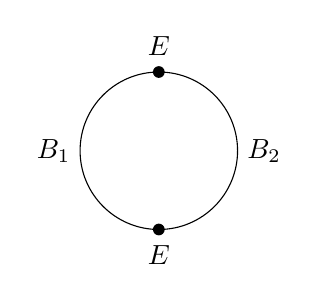
\begin{tikzpicture}[%every label/.style={green}
]
\node[fill=black, circle, label=below:$E$, inner sep=1.5pt](S) at (0,0) {};
\node[fill=black, circle, label=above:$E$, inner sep=1.5pt](N) at (0,2) {};
\draw (S) arc  (-90:90:1);
\draw (N) arc  (90:270:1);
\node[left] at (-1,1) {$B_1$};
\node[right] at (1,1) {$B_2$};
\end{tikzpicture}
\caption{Combining two balls to get a full boundary.}\label{blah3}\end{figure}

Note that we insist on injectivity above. 
The lemma follows from Definition \ref{def:colim-fields} and Lemma \ref{lem:colim-injective}.
%\nn{we might want a more official looking proof...}

We do not insist on surjectivity of the gluing map, since this is not satisfied by all of the examples
we are trying to axiomatize.
If our $k$-morphisms $\cC(X)$ are labeled cell complexes embedded in $X$ (c.f. Example \ref{ex:traditional-n-categories} below), then a $k$-morphism is
in the image of the gluing map precisely when the cell complex is in general position
with respect to $E$. On the other hand, in categories based on maps to a target space (c.f. Example \ref{ex:maps-to-a-space} below) the gluing map is always surjective.

If $S$ is a 0-sphere (the case $k=1$ above), then $S$ can be identified with the {\it disjoint} union
of two 0-balls $B_1$ and $B_2$ and the colimit construction $\cl{\cC}(S)$ can be identified
with the (ordinary, not fibered) product $\cC(B_1) \times \cC(B_2)$.

Let $\cl{\cC}(S)\trans E$ denote the image of $\gl_E$.
We will refer to elements of $\cl{\cC}(S)\trans E$ as ``splittable along $E$" or ``transverse to $E$". 
When the gluing map is surjective every such element is splittable.

If $X$ is a $k$-ball and $E \sub \bd X$ splits $\bd X$ into two $k{-}1$-balls $B_1$ and $B_2$
as above, then we define $\cC(X)\trans E = \bd^{-1}(\cl{\cC}(\bd X)\trans E)$.

We will call the projection $\cl{\cC}(S)\trans E \to \cC(B_i)$ given by the composition
$$\cl{\cC}(S)\trans E \xrightarrow{\gl^{-1}} \cC(B_1) \times \cC(B_2) \xrightarrow{\pr_i} \cC(B_i)$$
a {\it restriction} map and write $\res_{B_i}(a)$
(or simply $\res(a)$ when there is no ambiguity), for $a\in \cl{\cC}(S)\trans E$.
More generally, we also include under the rubric ``restriction map"
the boundary maps of Axiom \ref{nca-boundary} above,
another class of maps introduced after Axiom \ref{nca-assoc} below, as well as any composition
of restriction maps.
In particular, we have restriction maps $\cC(X)\trans E \to \cC(B_i)$
defined as the composition of the boundary with the first restriction map described above:
$$
\cC(X) \trans E \xrightarrow{\bdy} \cl{\cC}(\bdy X)\trans E \xrightarrow{\res} \cC(B_i)
.$$
These restriction maps can be thought of as 
domain and range maps, relative to the choice of splitting $\bd X = B_1 \cup_E B_2$.
These restriction maps in fact have their image in the subset $\cC(B_i)\trans E$,
and so to emphasize this we will sometimes write the restriction map as $\cC(X)\trans E \to \cC(B_i)\trans E$.


Next we consider composition of morphisms.
For $n$-categories which lack strong duality, one usually considers
$k$ different types of composition of $k$-morphisms, each associated to a different ``direction".
(For example, vertical and horizontal composition of 2-morphisms.)
In the presence of strong duality, these $k$ distinct compositions are subsumed into 
one general type of composition which can be in any direction.

\begin{axiom}[Composition]
\label{axiom:composition}
Let $B = B_1 \cup_Y B_2$, where $B$, $B_1$ and $B_2$ are $k$-balls ($0\le k\le n$)
and $Y = B_1\cap B_2$ is a $k{-}1$-ball (Figure \ref{blah5}).
Let $E = \bd Y$, which is a $k{-}2$-sphere.
Note that each of $B$, $B_1$ and $B_2$ has its boundary split into two $k{-}1$-balls by $E$.
We have restriction (domain or range) maps $\cC(B_i)\trans E \to \cC(Y)$.
Let $\cC(B_1)\trans E \times_{\cC(Y)} \cC(B_2)\trans E$ denote the fibered product of these two maps. 
We have a map
\[
	\gl_Y : \cC(B_1)\trans E \times_{\cC(Y)} \cC(B_2)\trans E \to \cC(B)\trans E
\]
which is natural with respect to the actions of homeomorphisms, and also compatible with restrictions
to the intersection of the boundaries of $B$ and $B_i$.
If $k < n$
we require that $\gl_Y$ is injective.
%(For $k=n$ see below.)
\end{axiom}

\begin{figure}[t] \centering
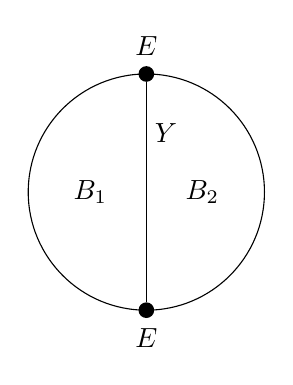
\begin{tikzpicture}[%every label/.style={green},
				x=1.5cm,y=1.5cm]
\node[fill=black, circle, label=below:$E$, inner sep=2pt](S) at (0,0) {};
\node[fill=black, circle, label=above:$E$, inner sep=2pt](N) at (0,2) {};
\draw (S) arc  (-90:90:1);
\draw (N) arc  (90:270:1);
\draw (N) -- (S);
\node[left] at (-1/4,1) {$B_1$};
\node[right] at (1/4,1) {$B_2$};
\node at (1/6,3/2)  {$Y$};
\end{tikzpicture}
\caption{From two balls to one ball.}\label{blah5}\end{figure}

\begin{axiom}[Strict associativity] \label{nca-assoc}
The composition (gluing) maps above are strictly associative.
Given any splitting of a ball $B$ into smaller balls
$$\bigsqcup B_i \to B,$$ 
any sequence of gluings (in the sense of Definition \ref{defn:gluing-decomposition}, where all the intermediate steps are also disjoint unions of balls) yields the same result.
\end{axiom}

\begin{figure}[t]
$$\mathfig{.65}{ncat/strict-associativity}$$
\caption{An example of strict associativity.}\label{blah6}\end{figure}

We'll use the notation  $a\bullet b$ for the glued together field $\gl_Y(a, b)$.
In the other direction, we will call the projection from $\cC(B)\trans E$ to $\cC(B_i)\trans E$ 
a restriction map (one of many types of map so called) and write $\res_{B_i}(a)$ for $a\in \cC(B)\trans E$.
%Compositions of boundary and restriction maps will also be called restriction maps.
%For example, if $B$ is a $k$-ball and $Y\sub \bd B$ is a $k{-}1$-ball, there is a
%restriction map from $\cC(B)_{\bd Y}$ to $\cC(Y)$.

We will write $\cC(B)\trans Y$ for the image of $\gl_Y$ in $\cC(B)$.
We will call elements of $\cC(B)\trans Y$ morphisms which are 
``splittable along $Y$'' or ``transverse to $Y$''.
We have $\cC(B)\trans Y \sub \cC(B)\trans E \sub \cC(B)$.

More generally, let $\alpha$ be a splitting of $X$ into smaller balls.
Let $\cC(X)_\alpha \sub \cC(X)$ denote the image of the iterated gluing maps from 
the smaller balls to $X$.
We  say that elements of $\cC(X)_\alpha$ are morphisms which are ``splittable along $\alpha$".
In situations where the splitting is notationally anonymous, we will write
$\cC(X)\spl$ for the morphisms which are splittable along (a.k.a.\ transverse to)
the unnamed splitting.
If $\beta$ is a ball decomposition of $\bd X$, we define $\cC(X)_\beta \deq \bd\inv(\cl{\cC}(\bd X)_\beta)$;
this can also be denoted $\cC(X)\spl$ if the context contains an anonymous
decomposition of $\bd X$ and no competing splitting of $X$.

The above two composition axioms are equivalent to the following one,
which we state in slightly vague form.

\xxpar{Multi-composition:}
{Given any splitting $B_1 \sqcup \cdots \sqcup B_m \to B$ of a $k$-ball
into small $k$-balls, there is a 
map from an appropriate subset (like a fibered product) 
of $\cC(B_1)\spl\times\cdots\times\cC(B_m)\spl$ to $\cC(B)\spl$,
and these various $m$-fold composition maps satisfy an
operad-type strict associativity condition (Figure \ref{fig:operad-composition}).}

\begin{figure}[t]
$$\mathfig{.8}{ncat/operad-composition}$$
\caption{Operad composition and associativity}\label{fig:operad-composition}\end{figure}

The next axiom is related to identity morphisms, though that might not be immediately obvious.

\begin{axiom}[Product (identity) morphisms, preliminary version]
For each $k$-ball $X$ and $m$-ball $D$, with $k+m \le n$, there is a map $\cC(X)\to \cC(X\times D)$, 
usually denoted $a\mapsto a\times D$ for $a\in \cC(X)$.
These maps must satisfy the following conditions.
\begin{enumerate}
\item
If $f:X\to X'$ and $\tilde{f}:X\times D \to X'\times D'$ are homeomorphisms such that the diagram
\[ \xymatrix{
	X\times D \ar[r]^{\tilde{f}} \ar[d]_{\pi} & X'\times D' \ar[d]^{\pi} \\
	X \ar[r]^{f} & X'
} \]
commutes, then we have 
\[
	\tilde{f}(a\times D) = f(a)\times D' .
\]
\item
Product morphisms are compatible with gluing (composition) in both factors:
\[
	(a'\times D)\bullet(a''\times D) = (a'\bullet a'')\times D
\]
and
\[
	(a\times D')\bullet(a\times D'') = a\times (D'\bullet D'') .
\]
\item
Product morphisms are associative:
\[
	(a\times D)\times D' = a\times (D\times D') .
\]
(Here we are implicitly using functoriality and the obvious homeomorphism
$(X\times D)\times D' \to X\times(D\times D')$.)
\item
Product morphisms are compatible with restriction:
\[
	\res_{X\times E}(a\times D) = a\times E
\]
for $E\sub \bd D$ and $a\in \cC(X)$.
\end{enumerate}
\end{axiom}

We will need to strengthen the above preliminary version of the axiom to allow
for products which are ``pinched" in various ways along their boundary.
(See Figure \ref{pinched_prods}.)
\begin{figure}[t]
$$
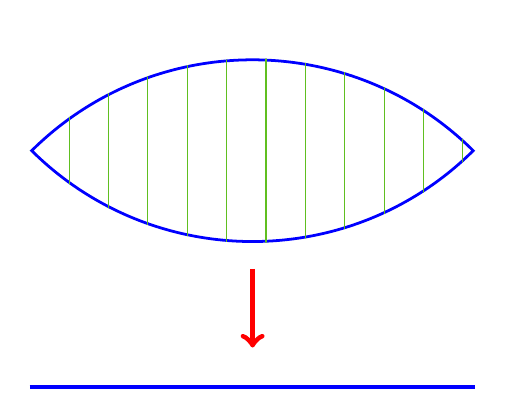
\begin{tikzpicture}[baseline=0]
\begin{scope}
\path[clip] (0,0) arc (135:45:4) arc (-45:-135:4);
\draw[blue,line width=2pt] (0,0) arc (135:45:4) arc (-45:-135:4);
\foreach \x in {0, 0.5, ..., 6} {
	\draw[green!50!brown] (\x,-2) -- (\x,2);
}
\end{scope}
\draw[blue,line width=1.5pt] (0,-3) -- (5.66,-3);
\draw[->,red,line width=2pt] (2.83,-1.5) -- (2.83,-2.5);
\end{tikzpicture}
\qquad \qquad
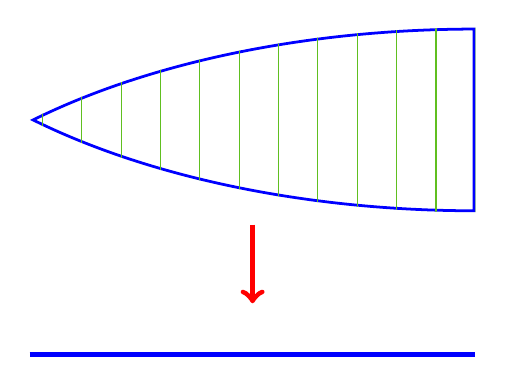
\begin{tikzpicture}[baseline=-0.15cm]
\begin{scope}
\path[clip] (0,1) arc (90:135:8 and 4)  arc (-135:-90:8 and 4) -- cycle;
\draw[blue,line width=2pt] (0,1) arc (90:135:8 and 4)  arc (-135:-90:8 and 4) -- cycle;
\foreach \x in {-6, -5.5, ..., 0} {
	\draw[green!50!brown] (\x,-2) -- (\x,2);
}
\end{scope}
\draw[blue,line width=1.5pt] (-5.66,-3.15) -- (0,-3.15);
\draw[->,red,line width=2pt] (-2.83,-1.5) -- (-2.83,-2.5);
\end{tikzpicture}
$$
\caption{Examples of pinched products}\label{pinched_prods}
\end{figure}
The need for a strengthened version will become apparent in Appendix \ref{sec:comparing-defs}
where we construct a traditional 2-category from a disk-like 2-category.
For example, ``half-pinched" products of 1-balls are used to construct weak identities for 1-morphisms
in 2-categories.
We also need fully-pinched products to define collar maps below (see Figure \ref{glue-collar}).

Define a {\it pinched product} to be a map
\[
	\pi: E\to X
\]
such that $E$ is a $k{+}m$-ball, $X$ is a $k$-ball ($m\ge 1$), and $\pi$ is locally modeled
on a standard iterated degeneracy map
\[
	d: \Delta^{k+m}\to\Delta^k .
\]
(We thank Kevin Costello for suggesting this approach.)

Note that for each interior point $x\in X$, $\pi\inv(x)$ is an $m$-ball,
and for each boundary point $x\in\bd X$, $\pi\inv(x)$ is a ball of dimension
$l \le m$, with $l$ depending on $x$.
It is easy to see that a composition of pinched products is again a pinched product.
A {\it sub pinched product} is a sub-$m$-ball $E'\sub E$ such that the restriction
$\pi:E'\to \pi(E')$ is again a pinched product.
A {union} of pinched products is a decomposition $E = \cup_i E_i$
such that each $E_i\sub E$ is a sub pinched product.
(See Figure \ref{pinched_prod_unions}.)
\begin{figure}[t]
$$
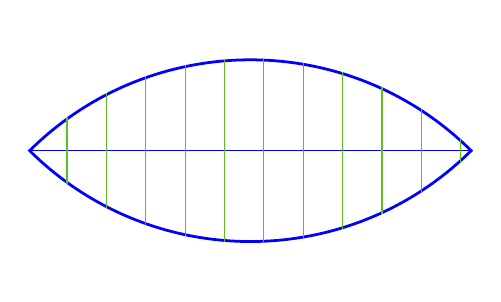
\begin{tikzpicture}[baseline=0]
\begin{scope}
\path[clip] (0,0) arc (135:45:4) arc (-45:-135:4);
\draw[blue,line width=2pt] (0,0) arc (135:45:4) arc (-45:-135:4);
\draw[blue] (0,0) -- (5.66,0);
\foreach \x in {0, 0.5, ..., 6} {
	\draw[green!50!brown] (\x,-2) -- (\x,2);
}
\end{scope}
\end{tikzpicture}
\qquad
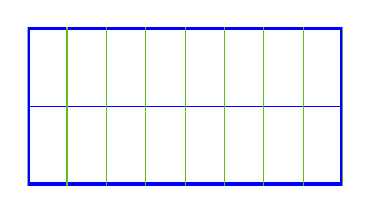
\begin{tikzpicture}[baseline=0]
\begin{scope}
\path[clip] (0,-1) rectangle (4,1);
\draw[blue,line width=2pt] (0,-1) rectangle (4,1);
\draw[blue] (0,0) -- (5,0);
\foreach \x in {0, 0.5, ..., 6} {
	\draw[green!50!brown] (\x,-2) -- (\x,2);
}
\end{scope}
\end{tikzpicture}
\qquad
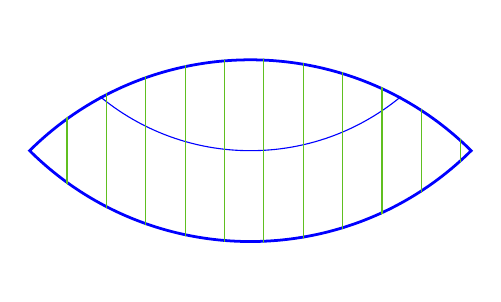
\begin{tikzpicture}[baseline=0]
\begin{scope}
\path[clip] (0,0) arc (135:45:4) arc (-45:-135:4);
\draw[blue,line width=2pt] (0,0) arc (135:45:4) arc (-45:-135:4);
\draw[blue] (2.83,3) circle (3);
\foreach \x in {0, 0.5, ..., 6} {
	\draw[green!50!brown] (\x,-2) -- (\x,2);
}
\end{scope}
\end{tikzpicture}
$$
$$
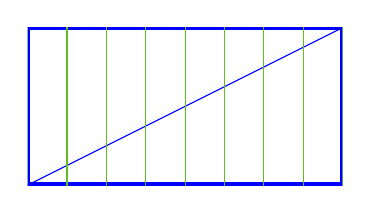
\begin{tikzpicture}[baseline=0]
\begin{scope}
\path[clip] (0,-1) rectangle (4,1);
\draw[blue,line width=2pt] (0,-1) rectangle (4,1);
\draw[blue] (0,-1) -- (4,1);
\foreach \x in {0, 0.5, ..., 6} {
	\draw[green!50!brown] (\x,-2) -- (\x,2);
}
\end{scope}
\end{tikzpicture}
\qquad
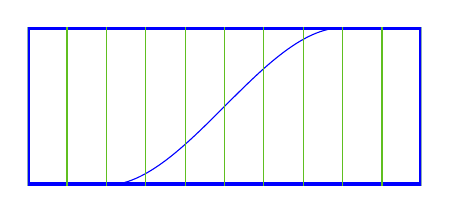
\begin{tikzpicture}[baseline=0]
\begin{scope}
\path[clip] (0,-1) rectangle (5,1);
\draw[blue,line width=2pt] (0,-1) rectangle (5,1);
\draw[blue] (1,-1) .. controls  (2,-1) and (3,1) .. (4,1);
\foreach \x in {0, 0.5, ..., 6} {
	\draw[green!50!brown] (\x,-2) -- (\x,2);
}
\end{scope}
\end{tikzpicture}
\qquad
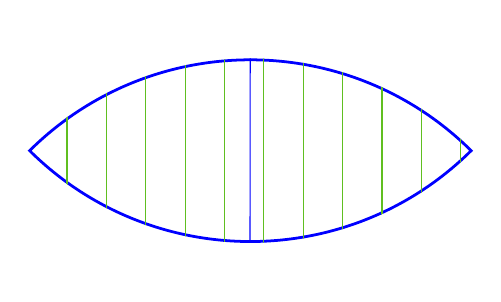
\begin{tikzpicture}[baseline=0]
\begin{scope}
\path[clip] (0,0) arc (135:45:4) arc (-45:-135:4);
\draw[blue,line width=2pt] (0,0) arc (135:45:4) arc (-45:-135:4);
\draw[blue] (2.82,-5) -- (2.83,5);
\foreach \x in {0, 0.5, ..., 6} {
	\draw[green!50!brown] (\x,-2) -- (\x,2);
}
\end{scope}
\end{tikzpicture}
$$
\caption{Six examples of unions of pinched products}\label{pinched_prod_unions}
\end{figure}

Note that $\bd X$ has a (possibly trivial) subdivision according to 
the dimension of $\pi\inv(x)$, $x\in \bd X$.
Let $\cC(X)\trans{}$ denote the morphisms which are splittable along this subdivision.

The product axiom will give a map $\pi^*:\cC(X)\trans{}\to \cC(E)$ for each pinched product
$\pi:E\to X$.
Morphisms in the image of $\pi^*$ will be called product morphisms.
Before stating the axiom, we illustrate it in our two motivating examples of $n$-categories.
In the case where $\cC(X) = \{f: X\to T\}$, we define $\pi^*(f) = f\circ\pi$.
In the case where $\cC(X)$ is the set of all labeled embedded cell complexes $K$ in $X$, 
define $\pi^*(K) = \pi\inv(K)$, with each codimension $i$ cell $\pi\inv(c)$ labeled by the
same (traditional) $i$-morphism as the corresponding codimension $i$ cell $c$.


%\addtocounter{axiom}{-1}
\begin{axiom}[Product (identity) morphisms]
\label{axiom:product}
For each pinched product $\pi:E\to X$, with $X$ a $k$-ball and $E$ a $k{+}m$-ball ($m\ge 1$),
there is a map $\pi^*:\cC(X)\trans{}\to \cC(E)$.
These maps must satisfy the following conditions.
\begin{enumerate}
\item
If $\pi:E\to X$ and $\pi':E'\to X'$ are pinched products, and
if $f:X\to X'$ and $\tilde{f}:E \to E'$ are maps such that the diagram
\[ \xymatrix{
	E \ar[r]^{\tilde{f}} \ar[d]_{\pi} & E' \ar[d]^{\pi'} \\
	X \ar[r]^{f} & X'
} \]
commutes, then we have 
\[
	\pi'^*\circ f = \tilde{f}\circ \pi^*.
\]
\item
Product morphisms are compatible with gluing (composition).
Let $\pi:E\to X$, $\pi_1:E_1\to X_1$, and $\pi_2:E_2\to X_2$ 
be pinched products with $E = E_1\cup E_2$.
(See Figure \ref{pinched_prod_unions}.)  
Note that $X_1$ and $X_2$ can be identified with subsets of $X$, 
but $X_1 \cap X_2$ might not be codimension 1, and indeed we might have $X_1 = X_2 = X$.
We assume that there is a decomposition of $X$ into balls which is compatible with
$X_1$ and $X_2$.
Let $a\in \cC(X)\trans{}$, and let $a_i$ denote the restriction of $a$ to $X_i\sub X$.
(We assume that $a$ is splittable with respect to the above decomposition of $X$ into balls.)
Then 
\[
	\pi^*(a) = \pi_1^*(a_1)\bullet \pi_2^*(a_2) .
\]
\item
Product morphisms are associative.
If $\pi:E\to X$ and $\rho:D\to E$ are pinched products then
\[
	\rho^*\circ\pi^* = (\pi\circ\rho)^* .
\]
\item
Product morphisms are compatible with restriction.
If we have a commutative diagram
\[ \xymatrix{
	D \ar@{^(->}[r] \ar[d]_{\rho} & E \ar[d]^{\pi} \\
	Y \ar@{^(->}[r] & X
} \]
such that $\rho$ and $\pi$ are pinched products, then
\[
	\res_D\circ\pi^* = \rho^*\circ\res_Y .
\]
\end{enumerate}
\end{axiom}


\medskip




%All of the axioms listed above hold for both ordinary $n$-categories and $A_\infty$ $n$-categories.
%The last axiom (below), concerning actions of 
%homeomorphisms in the top dimension $n$, distinguishes the two cases.

%We start with the ordinary $n$-category case.

The next axiom says, roughly, that we have strict associativity in dimension $n$, 
even when we reparametrize our $n$-balls.

\begin{axiom}[\textup{\textbf{[preliminary]}} Isotopy invariance in dimension $n$]
Let $X$ be an $n$-ball, $b \in \cC(X)$, and $f: X\to X$ be a homeomorphism which 
acts trivially on the restriction $\bd b$ of $b$ to $\bd X$.
(Keep in mind the important special case where $f$ restricted to $\bd X$ is the identity.)
Suppose furthermore that $f$ is isotopic to the identity through homeomorphisms which act
trivially on $\bd b$.
Then $f(b) = b$.
In particular, homeomorphisms which are isotopic to the identity rel boundary act trivially on 
all of $\cC(X)$.
\end{axiom}

This axiom needs to be strengthened to force product morphisms to act as the identity.
Let $X$ be an $n$-ball and $Y\sub\bd X$ be an $n{-}1$-ball.
Let $J$ be a 1-ball (interval).
Let $s_{Y,J}: X\cup_Y (Y\times J) \to X$ be a collaring homeomorphism
(see the end of \S\ref{ss:syst-o-fields}).
Here we use $Y\times J$ with boundary entirely pinched.
We define a map
\begin{eqnarray*}
	\psi_{Y,J}: \cC(X) &\to& \cC(X) \\
	a & \mapsto & s_{Y,J}(a \bullet ((a|_Y)\times J)) .
\end{eqnarray*}
(See Figure \ref{glue-collar}.)
\begin{figure}[t]
\begin{equation*}
\begin{tikzpicture}
\def\rad{1}
\def\srad{0.75}
\def\gap{4.5}
\foreach \i in {0, 1, 2} {
	\node(\i) at ($\i*(\gap,0)$) [draw, circle through = {($\i*(\gap,0)+(\rad,0)$)}] {};
	\node(\i-small) at (\i.east) [circle through={($(\i.east)+(\srad,0)$)}] {};
	\foreach \n in {1,2} {
		\fill (intersection \n of \i-small and \i) node(\i-intersection-\n) {} circle (2pt);
	}
}

\begin{scope}[decoration={brace,amplitude=10,aspect=0.5}]
	\draw[decorate] (0-intersection-1.east) -- (0-intersection-2.east);
\end{scope}
\node[right=1mm] at (0.east) {$a$};
\draw[->] ($(0.east)+(0.75,0)$) -- ($(1.west)+(-0.2,0)$);

\draw (1-small)  circle (\srad);
\foreach \theta in {90, 72, ..., -90} {
	\draw[blue] (1) -- ($(1)+(\rad,0)+(\theta:\srad)$);
}
\filldraw[fill=white] (1) circle (\rad);
\foreach \n in {1,2} {
	\fill (intersection \n of 1-small and 1) circle (2pt);
}
\node[below] at (1-small.south) {$a \times J$};
\draw[->] ($(1.east)+(1,0)$) -- ($(2.west)+(-0.2,0)$);

\begin{scope}
\path[clip] (2) circle (\rad);
\draw[clip] (2.east) circle (\srad);
\foreach \y in {1, 0.86, ..., -1} {
	\draw[blue] ($(2)+(-1,\y) $)-- ($(2)+(1,\y)$);
}
\end{scope}
\end{tikzpicture}
\end{equation*}
\begin{equation*}
\xymatrix@C+2cm{\cC(X) \ar[r]^(0.45){\text{glue}} & \cC(X \cup \text{collar}) \ar[r]^(0.55){\text{homeo}} & \cC(X)}
\end{equation*}

\caption{Extended homeomorphism.}\label{glue-collar}\end{figure}
We call a map of this form a {\it collar map}.
It can be thought of as the action of the inverse of
a map which projects a collar neighborhood of $Y$ onto $Y$,
or as the limit of homeomorphisms $X\to X$ which expand a very thin collar of $Y$
to a larger collar.
We call the equivalence relation generated by collar maps and homeomorphisms
isotopic (rel boundary) to the identity {\it extended isotopy}.

The revised axiom is

%\addtocounter{axiom}{-1}
\begin{axiom}[Extended isotopy invariance in dimension $n$]
\label{axiom:extended-isotopies}
Let $X$ be an $n$-ball, $b \in \cC(X)$, and $f: X\to X$ be a homeomorphism which 
acts trivially on the restriction $\bd b$ of $b$ to $\bd X$.
Suppose furthermore that $f$ is isotopic to the identity through homeomorphisms which
act trivially on $\bd b$.
Then $f(b) = b$.
In addition, collar maps act trivially on $\cC(X)$.
\end{axiom}

\medskip

We need one additional axiom.
It says, roughly, that given a $k$-ball $X$, $k<n$, and $c\in \cC(X)$, there exist sufficiently many splittings of $c$.
We use this axiom in the proofs of \ref{lem:d-a-acyclic}, \ref{lem:colim-injective} \nn{...}.
All of the examples of (disk-like) $n$-categories we consider in this paper satisfy the axiom, but
nevertheless we feel that it is too strong.
In the future we would like to see this provisional version of the axiom replaced by something less restrictive.

We give two alternate versions of he axiom, one better suited for smooth examples, and one better suited to PL examples.

\begin{axiom}[Splittings]
\label{axiom:splittings}
Let $c\in \cC_k(X)$, with $0\le k < n$.
Let $X = \cup_i X_i$ be a splitting of $X$.
\begin{itemize}
\item (Version 1) Then there exists an embedded cell complex $S_c \sub X$, called the string locus of $c$,
such that if the splitting $\{X_i\}$ is transverse to $S_c$ then $c$ splits along $\{X_i\}$.
\item (Version 2) Consider the set of homeomorphisms $g:X\to X$ such that $c$ splits along $\{g(X_i)\}$.
Then this subset of $\Homeo(X)$ is open and dense.
\end{itemize}
\nn{same something about extension from boundary}
\end{axiom}

We note some consequences of Axiom \ref{axiom:splittings}.

First, some preliminary definitions.
If $P$ is a poset let $P\times I$ denote the product poset, where $I = \{0, 1\}$ with ordering $0\le 1$.
Let $\Cone(P)$ denote $P$ adjoined an additional object $v$ (the vertex of the cone) with $p\le v$ for all objects $p$ of $P$.
Finally, let $\vcone(P)$ denote $P\times I \cup \Cone(P)$, where we identify $P\times \{0\}$ with the base of the cone.
We call $P\times \{1\}$ the base of $\vcone(P)$.
(See Figure \ref{vcone-fig}.)
\begin{figure}[t]
\centering
\begin{tikzpicture}
	[kw node/.style={circle,fill=orange!70},
	kw arrow/.style={-latex, very thick, blue!70, shorten >=.06cm, shorten <=.06cm},
	kw label/.style={cca},
	]

	\definecolor{cca}{rgb}{.1,.4,.3};

	\node at (0,0) {
		\begin{tikzpicture}	
			\draw 
				(0,0) node[kw node](p1){}
				(1,.5) node[kw node](p2){}
				(2,0) node[kw node](p3){};
			
			\draw[kw arrow] (p1) -- (p3);
			\draw[kw arrow] (p2) -- (p3);
			\draw[kw arrow] (p1) -- (p2);
			
			\draw[kw label] (1,-.6) node{(a)};
		\end{tikzpicture}
	};
	
	\node at (7,0) {
		\begin{tikzpicture}	
			\draw 
				(0,0) node[kw node](p1){}
				++(0,2.5) node[kw node](q1){}
				(1,.5) node[kw node](p2){}
				++(0,2.5) node[kw node](q2){}
				(2,0)  node[kw node](p3){}
				++(0,2.5) node[kw node](q3){}
				;
			
			\draw[kw arrow] (p1) -- (p3);
			\draw[kw arrow] (p2) -- (p3);
			\draw[kw arrow] (p1) -- (p2);
			\draw[kw arrow] (q1) -- (q3);
			\draw[kw arrow] (q2) -- (q3);
			\draw[kw arrow] (q1) -- (q2);
			\draw[kw arrow] (p1) -- (q1);
			\draw[kw arrow] (p2) -- (q2);
			\draw[kw arrow] (p3) -- (q3);

			\draw[kw label] (1,-.6) node{(b)};
		\end{tikzpicture}
	};
	
	\node at (0,-5) {
		\begin{tikzpicture}	
			\draw 
				(0,0) node[kw node](p1){}
				(1,.5) node[kw node](p2){}
				++(0,2.5) node[kw node](v){}
				(2,0)  node[kw node](p3){}
				;
			
			\draw[kw arrow] (p1) -- (p3);
			\draw[kw arrow] (p2) -- (p3);
			\draw[kw arrow] (p1) -- (p2);
			\draw[kw arrow] (p1) -- (v);
			\draw[kw arrow] (p2) -- (v);
			\draw[kw arrow] (p3) -- (v);

			\draw[kw label] (1,-.6) node{(c)};
		\end{tikzpicture}
	};
	
	\node at (7,-5) {
		\begin{tikzpicture}	
			\draw 
				(0,0) node[kw node](p1){}
				++(-2,2.5) node[kw node](q1){}
				(1,.5) node[kw node](p2){}
				++(-2,2.5) node[kw node](q2){}
				++(4,0) node[kw node](v){}
				(2,0)  node[kw node](p3){}
				++(-2,2.5) node[kw node](q3){}
				;
			
			\draw[kw arrow] (p1) -- (p3);
			\draw[kw arrow] (p2) -- (p3);
			\draw[kw arrow] (p1) -- (p2);
			\draw[kw arrow] (p1) -- (v);
			\draw[kw arrow] (p2) -- (v);
			\draw[kw arrow] (p3) -- (v);
			\draw[kw arrow] (q1) -- (q3);
			\draw[kw arrow] (q2) -- (q3);
			\draw[kw arrow] (q1) -- (q2);
			\draw[kw arrow] (p1) -- (q1);
			\draw[kw arrow] (p2) -- (q2);
			\draw[kw arrow] (p3) -- (q3);

			\draw[kw label] (1,-.6) node{(d)};
		\end{tikzpicture}
	};
	
\end{tikzpicture}
\caption{(a) $P$, (b) $P\times I$, (c) $\Cone(P)$, (d) $\vcone(P)$}
\label{vcone-fig}
\end{figure}


\begin{lem}
\label{lemma:vcones}
Let $c\in \cC_k(X)$, with $0\le k < n$, and
let $P$ be a finite poset of splittings of $c$.
Then we can embed $\vcone(P)$ into the splittings of $c$, with $P$ corresponding to the base of $\vcone(P)$.
Furthermore, if $q$ is any decomposition of $X$, then we can take the vertex of $\vcone(P)$ to be $q$ up to a small perturbation.
\end{lem}

\begin{proof}
After a small perturbation, we may assume that $q$ is simultaneously transverse to all the splittings in $P$, and
(by Axiom \ref{axiom:splittings}) that $c$ splits along $q$.
We can now choose, for each splitting $p$ in $P$, a common refinement $p'$ of $p$ and $q$.
This constitutes the middle part of $\vcone(P)$.
\end{proof}


\noop{ %%%%%%%%%%%%%%%%%%%%%%%%%%%%%%

We need one additional axiom, in order to constrain the poset of decompositions of a given morphism.
We will soon want to take colimits (and homotopy colimits) indexed by such posets, and we want to require
that these colimits are in some sense locally acyclic.
Before stating the axiom we need a few preliminary definitions.
If $P$ is a poset let $P\times I$ denote the product poset, where $I = \{0, 1\}$ with ordering $0\le 1$.
Let $\Cone(P)$ denote $P$ adjoined an additional object $v$ (the vertex of the cone) with $p\le v$ for all objects $p$ of $P$.
Finally, let $\vcone(P)$ denote $P\times I \cup \Cone(P)$, where we identify $P\times \{0\}$ with the base of the cone.
We call $P\times \{1\}$ the base of $\vcone(P)$.
(See Figure \ref{vcone-fig}.)
\begin{figure}[t]
\centering
\begin{tikzpicture}
	[kw node/.style={circle,fill=orange!70},
	kw arrow/.style={-latex, very thick, blue!70, shorten >=.06cm, shorten <=.06cm},
	kw label/.style={cca},
	]

	\definecolor{cca}{rgb}{.1,.4,.3};

	\node at (0,0) {
		\begin{tikzpicture}	
			\draw 
				(0,0) node[kw node](p1){}
				(1,.5) node[kw node](p2){}
				(2,0) node[kw node](p3){};
			
			\draw[kw arrow] (p1) -- (p3);
			\draw[kw arrow] (p2) -- (p3);
			\draw[kw arrow] (p1) -- (p2);
			
			\draw[kw label] (1,-.6) node{(a)};
		\end{tikzpicture}
	};
	
	\node at (7,0) {
		\begin{tikzpicture}	
			\draw 
				(0,0) node[kw node](p1){}
				++(0,2.5) node[kw node](q1){}
				(1,.5) node[kw node](p2){}
				++(0,2.5) node[kw node](q2){}
				(2,0)  node[kw node](p3){}
				++(0,2.5) node[kw node](q3){}
				;
			
			\draw[kw arrow] (p1) -- (p3);
			\draw[kw arrow] (p2) -- (p3);
			\draw[kw arrow] (p1) -- (p2);
			\draw[kw arrow] (q1) -- (q3);
			\draw[kw arrow] (q2) -- (q3);
			\draw[kw arrow] (q1) -- (q2);
			\draw[kw arrow] (p1) -- (q1);
			\draw[kw arrow] (p2) -- (q2);
			\draw[kw arrow] (p3) -- (q3);

			\draw[kw label] (1,-.6) node{(b)};
		\end{tikzpicture}
	};
	
	\node at (0,-5) {
		\begin{tikzpicture}	
			\draw 
				(0,0) node[kw node](p1){}
				(1,.5) node[kw node](p2){}
				++(0,2.5) node[kw node](v){}
				(2,0)  node[kw node](p3){}
				;
			
			\draw[kw arrow] (p1) -- (p3);
			\draw[kw arrow] (p2) -- (p3);
			\draw[kw arrow] (p1) -- (p2);
			\draw[kw arrow] (p1) -- (v);
			\draw[kw arrow] (p2) -- (v);
			\draw[kw arrow] (p3) -- (v);

			\draw[kw label] (1,-.6) node{(c)};
		\end{tikzpicture}
	};
	
	\node at (7,-5) {
		\begin{tikzpicture}	
			\draw 
				(0,0) node[kw node](p1){}
				++(-2,2.5) node[kw node](q1){}
				(1,.5) node[kw node](p2){}
				++(-2,2.5) node[kw node](q2){}
				++(4,0) node[kw node](v){}
				(2,0)  node[kw node](p3){}
				++(-2,2.5) node[kw node](q3){}
				;
			
			\draw[kw arrow] (p1) -- (p3);
			\draw[kw arrow] (p2) -- (p3);
			\draw[kw arrow] (p1) -- (p2);
			\draw[kw arrow] (p1) -- (v);
			\draw[kw arrow] (p2) -- (v);
			\draw[kw arrow] (p3) -- (v);
			\draw[kw arrow] (q1) -- (q3);
			\draw[kw arrow] (q2) -- (q3);
			\draw[kw arrow] (q1) -- (q2);
			\draw[kw arrow] (p1) -- (q1);
			\draw[kw arrow] (p2) -- (q2);
			\draw[kw arrow] (p3) -- (q3);

			\draw[kw label] (1,-.6) node{(d)};
		\end{tikzpicture}
	};
	
\end{tikzpicture}
\caption{(a) $P$, (b) $P\times I$, (c) $\Cone(P)$, (d) $\vcone(P)$}
\label{vcone-fig}
\end{figure}


\begin{axiom}[Splittings]
\label{axiom:vcones}
Let $c\in \cC_k(X)$, with $0\le k < n$, and
let $P$ be a finite poset of splittings of $c$.
Then we can embed $\vcone(P)$ into the splittings of $c$, with $P$ corresponding to the base of $\vcone(P)$.
Furthermore, if $q$ is any decomposition of $X$, then we can take the vertex of $\vcone(P)$ to be $q$ up to a small perturbation.
Also, any splitting of $\bd c$ can be extended to a splitting of $c$.
\end{axiom}

It is easy to see that this axiom holds in our two motivating examples, 
using standard facts about transversality and general position.
One starts with $q$, perturbs it so that it is in general position with respect to $c$ (in the case of string diagrams)
and also with respect to each of the decompositions of $P$, then chooses common refinements of each decomposition of $P$
and the perturbed $q$.
These common refinements form the middle ($P\times \{0\}$ above) part of $\vcone(P)$.

We note two simple special cases of Axiom \ref{axiom:vcones}.
If $P$ is the empty poset, then $\vcone(P)$ consists of only the vertex, and the axiom says that any morphism $c$
can be split along any decomposition of $X$, after a small perturbation.
If $P$ is the disjoint union of two points, then $\vcone(P)$ looks like a letter W, and the axiom implies that the
poset of splittings of $c$ is connected.
Note that we do not require that any two splittings of $c$ have a common refinement (i.e.\ replace the letter W with the letter V).
Two decompositions of $X$ might intersect in a very messy way, but one can always find a third
decomposition which has common refinements with each of the original two decompositions.

} %%%%%% end \noop %%%%%%%%%%%%%%%%%%%%%%%%%%%%

\medskip

This completes the definition of an $n$-category.
Next we define enriched $n$-categories.

\medskip


Most of the examples of $n$-categories we are interested in are enriched in the following sense.
The various sets of $n$-morphisms $\cC(X; c)$, for all $n$-balls $X$ and
all $c\in \cl{\cC}(\bd X)$, have the structure of an object in some appropriate auxiliary category
(e.g.\ vector spaces, or modules over some ring, or chain complexes),
and all the structure maps of the $n$-category are compatible with the auxiliary
category structure.
Note that this auxiliary structure is only in dimension $n$; if $\dim(Y) < n$ then 
$\cC(Y; c)$ is just a plain set.

%We will aim for a little bit more generality than we need and not assume that the objects
%of our auxiliary category are sets with extra structure.
First we must specify requirements for the auxiliary category.
It should have a {\it distributive monoidal structure} in the sense of 
\cite{1010.4527}.
This means that there is a monoidal structure $\otimes$ and also coproduct $\oplus$,
and these two structures interact in the appropriate way.
Examples include 
\begin{itemize}
\item vector spaces (or $R$-modules or chain complexes) with tensor product and direct sum; and
\item topological spaces with product and disjoint union.
\end{itemize}
For convenience, we will also assume that the objects of our auxiliary category are sets with extra structure.
(Otherwise, stating the axioms for identity morphisms becomes more cumbersome.)

Before stating the revised axioms for an $n$-category enriched in a distributive monoidal category,
we need a preliminary definition.
Once we have the above $n$-category axioms for $n{-}1$-morphisms, we can define the 
category $\bbc$ of {\it $n$-balls with boundary conditions}.
Its objects are pairs $(X, c)$, where $X$ is an $n$-ball and $c \in \cl\cC(\bd X)$ is the ``boundary condition".
The morphisms from $(X, c)$ to $(X', c')$, denoted $\Homeo(X,c; X', c')$, are
homeomorphisms $f:X\to X'$ such that $f|_{\bd X}(c) = c'$.
%Let $\pi_0(\bbc)$ denote
 
\begin{axiom}[Enriched $n$-categories]
\label{axiom:enriched}
Let $\cS$ be a distributive symmetric monoidal category.
An $n$-category enriched in $\cS$ satisfies the above $n$-category axioms for $k=0,\ldots,n-1$,
and modifies the axioms for $k=n$ as follows:
\begin{itemize}
\item Morphisms. We have a functor $\cC_n$ from $\bbc$ ($n$-balls with boundary conditions) to $\cS$.
%[already said this above.  ack]  Furthermore, $\cC_n(f)$ depends only on the path component of a homeomorphism $f: (X, c) \to (X', c')$.
%In particular, homeomorphisms which are isotopic to the identity rel boundary act trivially
\item Composition. Let $B = B_1\cup_Y B_2$ as in Axiom \ref{axiom:composition}.
Let $Y_i = \bd B_i \setmin Y$.  
Note that $\bd B = Y_1\cup Y_2$.
Let $c_i \in \cC(Y_i)$ with $\bd c_1 = \bd c_2 = d \in \cl\cC(E)$.
Then we have a map
\[
	\gl_Y : \bigoplus_c \cC(B_1; c_1 \bullet c) \otimes \cC(B_2; c_2\bullet c) \to \cC(B; c_1\bullet c_2),
\]
where the sum is over $c\in\cC(Y)$ such that $\bd c = d$.
This map is natural with respect to the action of homeomorphisms and with respect to restrictions.
%\item Product morphisms. \nn{Hmm... not sure what to say here. maybe we need sets with structure after all.}
\end{itemize}
\end{axiom}

\medskip

When the enriching category $\cS$ is chain complexes or topological spaces,
or more generally an appropriate sort of $\infty$-category,
we can modify the extended isotopy axiom \ref{axiom:extended-isotopies}
to require that families of homeomorphisms act
and obtain what we shall call an $A_\infty$ $n$-category.

\noop{
We believe that abstract definitions should be guided by diverse collections
of concrete examples, and a lack of diversity in our present collection of examples of $A_\infty$ $n$-categories
makes us reluctant to commit to an all-encompassing general definition.
Instead, we will give a relatively narrow definition which covers the examples we consider in this paper.
After stating it, we will briefly discuss ways in which it can be made more general.
}

Recall the category $\bbc$ of balls with boundary conditions.
Note that the morphisms $\Homeo(X,c; X', c')$ from $(X, c)$ to $(X', c')$ form a topological space.
Let $\cS$ be an appropriate $\infty$-category (e.g.\ chain complexes)
and let $\cJ$ be an $\infty$-functor from topological spaces to $\cS$
(e.g.\ the singular chain functor $C_*$).

\begin{axiom}[\textup{\textbf{[$A_\infty$ replacement for Axiom \ref{axiom:extended-isotopies}]}} Families of homeomorphisms act in dimension $n$.]
\label{axiom:families}
For each pair of $n$-balls $X$ and $X'$ and each pair $c\in \cl{\cC}(\bd X)$ and $c'\in \cl{\cC}(\bd X')$ we have an $\cS$-morphism
\[
	\cJ(\Homeo(X,c; X', c')) \ot \cC(X; c) \to \cC(X'; c') .
\]
Similarly, we have an $\cS$-morphism
\[
	\cJ(\Coll(X,c)) \ot \cC(X; c) \to \cC(X; c),
\]
where $\Coll(X,c)$ denotes the space of collar maps.
(See below for further discussion.)
These action maps are required to be associative up to coherent homotopy,
and also compatible with composition (gluing) in the sense that
a diagram like the one in Theorem \ref{thm:CH} commutes.
% say something about compatibility with product morphisms?
\end{axiom}

We now describe the topology on $\Coll(X; c)$.
We retain notation from the above definition of collar map.
Each collaring homeomorphism $X \cup (Y\times J) \to X$ determines a map from points $p$ of $\bd X$ to
(possibly length zero) embedded intervals in $X$ terminating at $p$.
If $p \in Y$ this interval is the image of $\{p\}\times J$.
If $p \notin Y$ then $p$ is assigned the length zero interval $\{p\}$.
Such collections of intervals have a natural topology, and $\Coll(X; c)$ inherits its topology from this.
Note in particular that parts of the collar are allowed to shrink continuously to zero length.
(This is the real content; if nothing shrinks to zero length then the action of families of collar
maps follows from the action of families of homeomorphisms and compatibility with gluing.)

The $k=n$ case of Axiom \ref{axiom:morphisms} posits a {\it strictly} associative action of {\it sets}
$\Homeo(X,c; X', c') \times \cC(X; c) \to \cC(X'; c')$, and at first it might seem that this would force the above
action of $\cJ(\Homeo(X,c; X', c'))$ to be strictly associative as well (assuming the two actions are compatible).
In fact, compatibility implies less than this.
For simplicity, assume that $\cJ$ is $C_*$, the singular chains functor.
(This is the example most relevant to this paper.)
Then compatibility implies that the action of $C_*(\Homeo(X,c; X', c'))$ agrees with the action
of $C_0(\Homeo(X,c; X', c'))$ coming from Axiom \ref{axiom:morphisms}, so we only require associativity in degree zero.
And indeed, this is true for our main example of an $A_\infty$ $n$-category based on the blob construction.
Stating this sort of compatibility for general $\cS$ and $\cJ$ requires further assumptions, 
such as the forgetful functor from $\cS$ to sets having a left adjoint, and $\cS$ having an internal Hom.

An alternative (due to Peter Teichner) is to say that Axiom \ref{axiom:families} 
supersedes the $k=n$ case of Axiom \ref{axiom:morphisms}; in dimension $n$ we just have a
functor $\bbc \to \cS$ of $A_\infty$ 1-categories.
(This assumes some prior notion of $A_\infty$ 1-category.)
We are not currently aware of any examples which require this sort of greater generality, so we think it best
to refrain from settling on a preferred version of the axiom until
we have a greater variety of examples to guide the choice.

Note that if we think of an ordinary 1-category as an $A_\infty$ 1-category where $k$-morphisms are identities for $k>1$,
then Axiom \ref{axiom:families} implies Axiom \ref{axiom:extended-isotopies}.

Another variant of the above axiom would be to drop the ``up to homotopy" and require a strictly associative action. 
In fact, the alternative construction $\btc_*(X)$ of the blob complex described in \S \ref{ss:alt-def} 
gives $n$-categories as in Example \ref{ex:blob-complexes-of-balls} which satisfy this stronger axiom. 
%since that construction is only homotopy equivalent to the usual one, only the weaker axiom carries across.
For future reference we make the following definition.

\begin{defn}
A {\em strict $A_\infty$ $n$-category} is one in which the actions of Axiom \ref{axiom:families} are strictly associative.
\end{defn}

\noop{
Note that if we take homology of chain complexes, we turn an $A_\infty$ $n$-category
into a ordinary $n$-category (enriched over graded groups).
In a different direction, if we enrich over topological spaces instead of chain complexes,
we get a space version of an $A_\infty$ $n$-category, with $\Homeo_\bd(X)$ acting 
instead of  $C_*(\Homeo_\bd(X))$.
Taking singular chains converts such a space type $A_\infty$ $n$-category into a chain complex
type $A_\infty$ $n$-category.
}


\medskip

We define a $j$ times monoidal $n$-category to be an $(n{+}j)$-category $\cC$ where
$\cC(X)$ is a trivial 1-element set if $X$ is a $k$-ball with $k<j$.
See Example \ref{ex:bord-cat}.

\medskip

The alert reader will have already noticed that our definition of an (ordinary) $n$-category
is extremely similar to our definition of a system of fields.
There are two differences.
First, for the $n$-category definition we restrict our attention to balls
(and their boundaries), while for fields we consider all manifolds.
Second,  in the category definition we directly impose isotopy
invariance in dimension $n$, while in the fields definition we 
instead remember a subspace of local relations which contain differences of isotopic fields. 
(Recall that the compensation for this complication is that we can demand that the gluing map for fields is injective.)
Thus a system of fields and local relations $(\cF,U)$ determines an $n$-category $\cC_ {\cF,U}$ simply by restricting our attention to
balls and, at level $n$, quotienting out by the local relations:
\begin{align*}
\cC_{\cF,U}(B^k) & = \begin{cases}\cF(B) & \text{when $k<n$,} \\ \cF(B) / U(B) & \text{when $k=n$.}\end{cases}
\end{align*}
This $n$-category can be thought of as the local part of the fields.
Conversely, given a disk-like $n$-category we can construct a system of fields via 
a colimit construction; see \S \ref{ss:ncat_fields} below.

\medskip

In the $n$-category axioms above we have intermingled data and properties for expository reasons.
Here's a summary of the definition which segregates the data from the properties.
We also remind the reader of the inductive nature of the definition: All the data for $k{-}1$-morphisms must be in place
before we can describe the data for $k$-morphisms.

An $n$-category consists of the following data:
\begin{itemize}
\item functors $\cC_k$ from $k$-balls to sets, $0\le k\le n$ (Axiom \ref{axiom:morphisms});
\item boundary natural transformations $\cC_k \to \cl{\cC}_{k-1} \circ \bd$ (Axiom \ref{nca-boundary});
\item ``composition'' or ``gluing'' maps $\gl_Y : \cC(B_1)\trans E \times_{\cC(Y)} \cC(B_2)\trans E \to \cC(B_1\cup_Y B_2)\trans E$ (Axiom \ref{axiom:composition});
\item ``product'' or ``identity'' maps $\pi^*:\cC(X)\to \cC(E)$ for each pinched product $\pi:E\to X$ (Axiom \ref{axiom:product});
\item if enriching in an auxiliary category, additional structure on $\cC_n(X; c)$ (Axiom \ref{axiom:enriched});
%\item in the $A_\infty$ case, an action of $C_*(\Homeo_\bd(X))$, and similarly for families of collar maps (Axiom \ref{axiom:families}).
\item in the $A_\infty$ case, actions of the topological spaces of homeomorphisms preserving boundary conditions
and collar maps (Axiom \ref{axiom:families}).
\end{itemize}
The above data must satisfy the following conditions.
\begin{itemize}
\item The gluing maps are compatible with actions of homeomorphisms and boundary 
restrictions (Axiom \ref{axiom:composition}).
\item For $k<n$ the gluing maps are injective (Axiom \ref{axiom:composition}).
\item The gluing maps are strictly associative (Axiom \ref{nca-assoc}).
\item The product maps are associative and also compatible with homeomorphism actions, gluing and restriction (Axiom \ref{axiom:product}).
\item If enriching in an auxiliary category, all of the data should be compatible 
with the auxiliary category structure on $\cC_n(X; c)$ (Axiom \ref{axiom:enriched}).
\item The possible splittings of a morphism satisfy various conditions (Axiom \ref{axiom:splittings}).
\item For ordinary categories, invariance of $n$-morphisms under extended isotopies 
and collar maps (Axiom \ref{axiom:extended-isotopies}).
\end{itemize}


\subsection{Examples of \texorpdfstring{$n$}{n}-categories}
\label{ss:ncat-examples}


We now describe several classes of examples of $n$-categories satisfying our axioms.
We typically specify only the morphisms; the rest of the data for the category
(restriction maps, gluing, product morphisms, action of homeomorphisms) is usually obvious.

\begin{example}[Maps to a space]
\rm
\label{ex:maps-to-a-space}%
Let $T$ be a topological space.
We define $\pi_{\leq n}(T)$, the fundamental $n$-category of $T$, as follows.
For $X$ a $k$-ball with $k < n$, define $\pi_{\leq n}(T)(X)$ to be the set of 
all continuous maps from $X$ to $T$.
For $X$ an $n$-ball define $\pi_{\leq n}(T)(X)$ to be continuous maps from $X$ to $T$ modulo
homotopies fixed on $\bd X$.
(Note that homotopy invariance implies isotopy invariance.)
For $a\in \cC(X)$ define the product morphism $a\times D \in \cC(X\times D)$ to
be $a\circ\pi_X$, where $\pi_X : X\times D \to X$ is the projection.
\end{example}

\noop{
Recall we described a system of fields and local relations based on maps to $T$ in Example \ref{ex:maps-to-a-space(fields)} above.
Constructing a system of fields from $\pi_{\leq n}(T)$ recovers that example.
\nn{shouldn't this go elsewhere?  we haven't yet discussed constructing a system of fields from
an n-cat}
}

\begin{example}[Maps to a space, with a fiber] \label{ex:maps-with-fiber}
\rm
\label{ex:maps-to-a-space-with-a-fiber}%
We can modify the example above, by fixing a
closed $m$-manifold $F$, and defining $\pi^{\times F}_{\leq n}(T)(X) = \Maps(X \times F \to T)$, 
otherwise leaving the definition in Example \ref{ex:maps-to-a-space} unchanged.
Taking $F$ to be a point recovers the previous case.
\end{example}

\begin{example}[Linearized, twisted, maps to a space]
\rm
\label{ex:linearized-maps-to-a-space}%
We can linearize Examples \ref{ex:maps-to-a-space} and \ref{ex:maps-to-a-space-with-a-fiber} as follows.
Let $\alpha$ be an $(n{+}m{+}1)$-cocycle on $T$ with values in a ring $R$
(have in mind the trivial cocycle).
For $X$ of dimension less than $n$ define $\pi^{\alpha, \times F}_{\leq n}(T)(X)$ as before, ignoring $\alpha$.
For $X$ an $n$-ball and $c\in \Maps(\bdy X \times F \to T)$ define $\pi^{\alpha, \times F}_{\leq n}(T)(X; c)$ to be
the $R$-module of finite linear combinations of continuous maps from $X\times F$ to $T$,
modulo the relation that if $a$ is homotopic to $b$ (rel boundary) via a homotopy
$h: X\times F\times I \to T$, then $a = \alpha(h)b$.
(In order for this to be well-defined we must choose $\alpha$ to be zero on degenerate simplices.
Alternatively, we could equip the balls with fundamental classes.)
\end{example}

\begin{example}[$n$-categories from TQFTs]
\rm
\label{ex:ncats-from-tqfts}%
Let $\cF$ be a TQFT in the sense of \S\ref{sec:fields}: an $n$-dimensional 
system of fields (also denoted $\cF$) and local relations.
Let $W$ be an $n{-}j$-manifold.
Define the $j$-category $\cF(W)$ as follows.
If $X$ is a $k$-ball with $k<j$, let $\cF(W)(X) \deq \cF(W\times X)$.
If $X$ is a $j$-ball and $c\in \cl{\cF(W)}(\bd X)$, 
let $\cF(W)(X; c) \deq A_\cF(W\times X; c)$.
\end{example}

The next example is only intended to be illustrative, as we don't specify 
which definition of a ``traditional $n$-category" we intend.
Further, most of these definitions don't even have an agreed-upon notion of 
``strong duality", which we assume here.
\begin{example}[Traditional $n$-categories]
\rm
\label{ex:traditional-n-categories}
Given a ``traditional $n$-category with strong duality" $C$
define $\cC(X)$, for $X$ a $k$-ball with $k < n$,
to be the set of all $C$-labeled embedded cell complexes of $X$ (c.f. \S \ref{sec:fields}).
For $X$ an $n$-ball and $c\in \cl{\cC}(\bd X)$, define $\cC(X; c)$ to be finite linear
combinations of $C$-labeled embedded cell complexes of $X$
modulo the kernel of the evaluation map.
Define a product morphism $a\times D$, for $D$ an $m$-ball, to be the product of the cell complex of $a$ with $D$,
with each cell labelled according to the corresponding cell for $a$.
(These two cells have the same codimension.)
More generally, start with an $n{+}m$-category $C$ and a closed $m$-manifold $F$.
Define $\cC(X)$, for $\dim(X) < n$,
to be the set of all $C$-labeled embedded cell complexes of $X\times F$.
Define $\cC(X; c)$, for $X$ an $n$-ball,
to be the dual Hilbert space $A(X\times F; c)$.
(See \S\ref{sec:constructing-a-tqft}.)
\end{example}


\begin{example}[The bordism $n$-category of $d$-manifolds, ordinary version]
\label{ex:bord-cat}
\rm
\label{ex:bordism-category}
For a $k$-ball $X$, $k<n$, define $\Bord^{n,d}(X)$ to be the set of all $(d{-}n{+}k)$-dimensional PL
submanifolds $W$ of $X\times \Real^\infty$ such that $\bd W = W \cap \bd X \times \Real^\infty$.
For an $n$-ball $X$ define $\Bord^{n,d}(X)$ to be homeomorphism classes (rel boundary) of such $d$-dimensional submanifolds;
we identify $W$ and $W'$ if $\bd W = \bd W'$ and there is a homeomorphism
$W \to W'$ which restricts to the identity on the boundary.
For $n=1$ we have the familiar bordism 1-category of $d$-manifolds.
The case $n=d$ captures the $n$-categorical nature of bordisms.
The case $n > 2d$ captures the full symmetric monoidal $n$-category structure.
\end{example}
\begin{rem}
Working with the smooth bordism category would require careful attention to either collars, corners or halos.
\end{rem}

%\nn{the next example might be an unnecessary distraction.  consider deleting it.}

%\begin{example}[Variation on the above examples]
%We could allow $F$ to have boundary and specify boundary conditions on $X\times \bd F$,
%for example product boundary conditions or take the union over all boundary conditions.
%%\nn{maybe should not emphasize this case, since it's ``better" in some sense
%%to think of these guys as affording a representation
%%of the $n{+}1$-category associated to $\bd F$.}
%\end{example}


%We have two main examples of $A_\infty$ $n$-categories, coming from maps to a target space and from the blob complex.

\begin{example}[Chains (or space) of maps to a space]
\rm
\label{ex:chains-of-maps-to-a-space}
We can modify Example \ref{ex:maps-to-a-space} above to define the fundamental $A_\infty$ $n$-category $\pi^\infty_{\le n}(T)$ of a topological space $T$.
For a $k$-ball $X$, with $k < n$, the set $\pi^\infty_{\leq n}(T)(X)$ is just $\Maps(X \to T)$.
Define $\pi^\infty_{\leq n}(T)(X; c)$ for an $n$-ball $X$ and $c \in \pi^\infty_{\leq n}(T)(\bdy X)$ to be the chain complex
\[
	C_*(\Maps_c(X \to T)),
\]
where $\Maps_c$ denotes continuous maps restricting to $c$ on the boundary,
and $C_*$ denotes singular chains.
Alternatively, if we take the $n$-morphisms to be simply $\Maps_c(X \to T)$, 
we get an $A_\infty$ $n$-category enriched over spaces.
\end{example}

See also Theorem \ref{thm:map-recon} below, recovering $C_*(\Maps(M \to T))$ up to 
homotopy as the blob complex of $M$ with coefficients in $\pi^\infty_{\le n}(T)$.

\begin{example}[Blob complexes of balls (with a fiber)]
\rm
\label{ex:blob-complexes-of-balls}
Fix an $n{-}k$-dimensional manifold $F$ and an $n$-dimensional system of fields $\cE$.
We will define an $A_\infty$ $k$-category $\cC$.
When $X$ is an $m$-ball, with $m<k$, define $\cC(X) = \cE(X\times F)$.
When $X$ is a $k$-ball,
define $\cC(X; c) = \bc^\cE_*(X\times F; c)$
where $\bc^\cE_*$ denotes the blob complex based on $\cE$.
\end{example}

This example will be used in Theorem \ref{thm:product} below, which allows us to compute the blob complex of a product.
Notice that with $F$ a point, the above example is a construction turning an ordinary 
$n$-category $\cC$ into an $A_\infty$ $n$-category.
We think of this as providing a ``free resolution" 
of the ordinary $n$-category. 
%\nn{say something about cofibrant replacements?}
In fact, there is also a trivial, but mostly uninteresting, way to do this: 
we can think of each vector space associated to an $n$-ball as a chain complex concentrated in degree $0$, 
and take $\CD{B}$ to act trivially. 

Beware that the ``free resolution" of the ordinary $n$-category $\pi_{\leq n}(T)$ 
is not the $A_\infty$ $n$-category $\pi^\infty_{\leq n}(T)$.
It's easy to see that with $n=0$, the corresponding system of fields is just 
linear combinations of connected components of $T$, and the local relations are trivial.
There's no way for the blob complex to magically recover all the data of $\pi^\infty_{\leq 0}(T) \iso C_* T$.

\begin{example}[The bordism $n$-category of $d$-manifolds, $A_\infty$ version]
\rm
\label{ex:bordism-category-ainf}
As in Example \ref{ex:bord-cat}, for $X$ a $k$-ball, $k<n$, we define $\Bord^{n,d}_\infty(X)$
to be the set of all $(d{-}n{+}k)$-dimensional
submanifolds $W$ of $X\times \Real^\infty$ such that $\bd W = W \cap \bd X \times \Real^\infty$.
For an $n$-ball $X$ with boundary condition $c$ 
define $\Bord^{n,d}_\infty(X; c)$ to be the space of all $d$-dimensional
submanifolds $W$ of $X\times \Real^\infty$ such that 
$W$ coincides with $c$ at $\bd X \times \Real^\infty$.
(The topology on this space is induced by ambient isotopy rel boundary.
This is homotopy equivalent to a disjoint union of copies $\mathrm{B}\!\Homeo(W')$, where
$W'$ runs though representatives of homeomorphism types of such manifolds.)
\end{example}



Let $\cE\cB_n$ be the operad of smooth embeddings of $k$ (little)
copies of the standard $n$-ball $B^n$ into another (big) copy of $B^n$.
(We require that the interiors of the little balls be disjoint, but their 
boundaries are allowed to meet.
Note in particular that the space for $k=1$ contains a copy of $\Diff(B^n)$, namely
the embeddings of a ``little" ball with image all of the big ball $B^n$.
(But note also that this inclusion is not
necessarily a homotopy equivalence.))
The operad $\cE\cB_n$ is homotopy equivalent to the standard framed little $n$-ball operad:
by shrinking the little balls (precomposing them with dilations), 
we see that both operads are homotopic to the space of $k$ framed points
in $B^n$.
It is easy to see that $n$-fold loop spaces $\Omega^n(T)$  have
an action of $\cE\cB_n$.
%\nn{add citation for this operad if we can find one}

\begin{example}[$E_n$ algebras]
\rm
\label{ex:e-n-alg}
Let $A$ be an $\cE\cB_n$-algebra.
Note that this implies a $\Diff(B^n)$ action on $A$, 
since $\cE\cB_n$ contains a copy of $\Diff(B^n)$.
We will define a strict $A_\infty$ $n$-category $\cC^A$.
(We enrich in topological spaces, though this could easily be adapted to, say, chain complexes.)
If $X$ is a ball of dimension $k<n$, define $\cC^A(X)$ to be a point.
In other words, the $k$-morphisms are trivial for $k<n$.
If $X$ is an $n$-ball, we define $\cC^A(X)$ via a colimit construction.
(Plain colimit, not homotopy colimit.)
Let $J$ be the category whose objects are embeddings of a disjoint union of copies of 
the standard ball $B^n$ into $X$, and whose morphisms are given by engulfing some of the 
embedded balls into a single larger embedded ball.
To each object of $J$ we associate $A^{\times m}$ (where $m$ is the number of balls), and
to each morphism of $J$ we associate a morphism coming from the $\cE\cB_n$ action on $A$.
Alternatively and more simply, we could define $\cC^A(X)$ to be 
$\Diff(B^n\to X)\times A$ modulo the diagonal action of $\Diff(B^n)$.
The remaining data for the $A_\infty$ $n$-category 
--- composition and $\Diff(X\to X')$ action ---
also comes from the $\cE\cB_n$ action on $A$.
%\nn{should we spell this out?}

Conversely, one can show that a disk-like strict $A_\infty$ $n$-category $\cC$, where the $k$-morphisms
$\cC(X)$ are trivial (single point) for $k<n$, gives rise to 
an $\cE\cB_n$-algebra.
%\nn{The paper is already long; is it worth giving details here?}
% According to the referee, yes it is...
Let $A = \cC(B^n)$, where $B^n$ is the standard $n$-ball.
We must define maps
\[
	\cE\cB_n^k \times A \times \cdots \times A \to A ,
\]
where $\cE\cB_n^k$ is the $k$-th space of the $\cE\cB_n$ operad.
Let $(b, a_1,\ldots,a_k)$ be a point of $\cE\cB_n^k \times A \times \cdots \times A \to A$.
The $i$-th embedding of $b$ together with $a_i$ determine an element of $\cC(B_i)$, 
where $B_i$ denotes the $i$-th little ball.
Using composition of $n$-morphsims in $\cC$, and padding the spaces between the little balls with the 
(essentially unique) identity $n$-morphism of $\cC$, we can construct a well-defined element
of $\cC(B^n) = A$.

If we apply the homotopy colimit construction of the next subsection to this example, 
we get an instance of Lurie's topological chiral homology construction.
\end{example}


\subsection{From balls to manifolds}
\label{ss:ncat_fields} \label{ss:ncat-coend}
In this section we show how to extend an $n$-category $\cC$ as described above 
(of either the ordinary or $A_\infty$ variety) to an invariant of manifolds, which we denote by $\cl{\cC}$.
This extension is a certain colimit, and the arrow in the notation is intended as a reminder of this.

In the case of ordinary $n$-categories, this construction factors into a construction of a 
system of fields and local relations, followed by the usual TQFT definition of a 
vector space invariant of manifolds given as Definition \ref{defn:TQFT-invariant}.
For an $A_\infty$ $n$-category, $\cl{\cC}$ is defined using a homotopy colimit instead.
Recall that we can take an ordinary $n$-category $\cC$ and pass to the ``free resolution", 
an $A_\infty$ $n$-category $\bc_*(\cC)$, by computing the blob complex of balls 
(recall Example \ref{ex:blob-complexes-of-balls} above).
We will show in Corollary \ref{cor:new-old} below that the homotopy colimit invariant 
for a manifold $M$ associated to this $A_\infty$ $n$-category is actually the 
same as the original blob complex for $M$ with coefficients in $\cC$.

Recall that we've already anticipated this construction Subsection \ref{ss:n-cat-def}, 
inductively defining $\cl{\cC}$ on $k$-spheres in terms of $\cC$ on $k$-balls, 
so that we can state the boundary axiom for $\cC$ on $k+1$-balls.

\medskip

We will first define the {\it decomposition poset} $\cell(W)$ for any $k$-manifold $W$, for $1 \leq k \leq n$. 
An $n$-category $\cC$ provides a functor from this poset to the category of sets, 
and we  will define $\cl{\cC}(W)$ as a suitable colimit 
(or homotopy colimit in the $A_\infty$ case) of this functor. 
We'll later give a more explicit description of this colimit.
In the case that the $n$-category $\cC$ is enriched (e.g. associates vector spaces or chain 
complexes to $n$-balls with boundary data), 
then the resulting colimit is also enriched, that is, the set associated to $W$ splits into 
subsets according to boundary data, and each of these subsets has the appropriate structure 
(e.g. a vector space or chain complex).

Recall (Definition \ref{defn:gluing-decomposition}) that a {\it ball decomposition} of $W$ is a 
sequence of gluings $M_0\to M_1\to\cdots\to M_m = W$ such that $M_0$ is a disjoint union of balls
$\du_a X_a$.
Abusing notation, we let $X_a$ denote both the ball (component of $M_0$) and
its image in $W$ (which is not necessarily a ball --- parts of $\bd X_a$ may have been glued together).
Define a {\it permissible decomposition} of $W$ to be a map
\[
	\coprod_a X_a \to W,
\]
which can be completed to a ball decomposition $\du_a X_a = M_0\to\cdots\to M_m = W$.
We further require that $\du_a (X_a \cap \bd W) \to \bd W$ 
can be completed to a (not necessarily ball) decomposition of $\bd W$.
(So, for example, in Example \ref{sin1x-example} if we take $W = B\cup C\cup D$ then $B\du C\du D \to W$
is not allowed since $D\cap \bd W$ is not a submanifold.)
Roughly, a permissible decomposition is like a ball decomposition where we don't care in which order the balls
are glued up to yield $W$, so long as there is some (non-pathological) way to glue them.

(Every smooth or PL manifold has a ball decomposition, but certain topological manifolds (e.g.\ non-smoothable
topological 4-manifolds) do not have ball decompositions.
For such manifolds we have only the empty colimit.)

We want the category (poset) of decompositions of $W$ to be small, so when we say decomposition we really
mean isomorphism class of decomposition.
Isomorphisms are defined in the obvious way: a collection of homeomorphisms $M_i\to M_i'$ which commute
with the gluing maps $M_i\to M_{i+1}$ and $M'_i\to M'_{i+1}$.

Given permissible decompositions $x = \{X_a\}$ and $y = \{Y_b\}$ of $W$, we say that $x$ is a refinement
of $y$, or write $x \le y$, if there is a ball decomposition $\du_a X_a = M_0\to\cdots\to M_m = W$
with $\du_b Y_b = M_i$ for some $i$,
and with $M_0, M_1, \ldots, M_i$ each being a disjoint union of balls.

\begin{defn}
The poset $\cell(W)$ has objects the permissible decompositions of $W$, 
and a unique morphism from $x$ to $y$ if and only if $x$ is a refinement of $y$.
See Figure \ref{partofJfig}.
\end{defn}

\begin{figure}[t]
\begin{equation*}
\mathfig{.63}{ncat/zz2}
\end{equation*}
\caption{A small part of $\cell(W)$}
\label{partofJfig}
\end{figure}

An $n$-category $\cC$ determines 
a functor $\psi_{\cC;W}$ from $\cell(W)$ to the category of sets 
(possibly with additional structure if $k=n$).
Let $x = \{X_a\}$ be a permissible decomposition of $W$ (i.e.\ object of $\cD(W)$).
We will define $\psi_{\cC;W}(x)$ to be a certain subset of $\prod_a \cC(X_a)$.
Roughly speaking, $\psi_{\cC;W}(x)$ is the subset where the restriction maps from
$\cC(X_a)$ and $\cC(X_b)$ agree whenever some part of $\bd X_a$ is glued to some part of $\bd X_b$.
(Keep in mind that perhaps $a=b$.)
Since we allow decompositions in which the intersection of $X_a$ and $X_b$ might be messy 
(see Example \ref{sin1x-example}), we must define $\psi_{\cC;W}(x)$ in a more roundabout way.

Inductively, we may assume that we have already defined the colimit $\cl\cC(M)$ for $k{-}1$-manifolds $M$.
(To start the induction, we define $\cl\cC(M)$, where $M = \du_a P_a$ is a 0-manifold and each $P_a$ is
a 0-ball, to be $\prod_a \cC(P_a)$.)
We also assume, inductively, that we have gluing and restriction maps for colimits of $k{-}1$-manifolds.
Gluing and restriction maps for colimits of $k$-manifolds will be defined later in this subsection.

Let $\du_a X_a = M_0\to\cdots\to M_m = W$ be a ball decomposition compatible with $x$.
Let $\bd M_i = N_i \cup Y_i \cup Y'_i$, where $Y_i$ and $Y'_i$ are glued together to produce $M_{i+1}$.
We will define $\psi_{\cC;W}(x)$ to be the subset of $\prod_a \cC(X_a)$ which satisfies a series of conditions
related to the gluings $M_{i-1} \to M_i$, $1\le i \le m$.
By Axiom \ref{nca-boundary}, we have a map
\[
	\prod_a \cC(X_a) \to \cl\cC(\bd M_0) .
\]
The first condition is that the image of $\psi_{\cC;W}(x)$ in $\cl\cC(\bd M_0)$ is splittable
along $\bd Y_0$ and $\bd Y'_0$, and that the restrictions to $\cl\cC(Y_0)$ and $\cl\cC(Y'_0)$ agree
(with respect to the identification of $Y_0$ and $Y'_0$ provided by the gluing map). 

On the subset of $\prod_a \cC(X_a)$ which satisfies the first condition above, we have a restriction
map to $\cl\cC(N_0)$ which we can compose with the gluing map 
$\cl\cC(N_0) \to \cl\cC(\bd M_1)$.
The second condition is that the image of $\psi_{\cC;W}(x)$ in $\cl\cC(\bd M_1)$ is splittable
along $\bd Y_1$ and $\bd Y'_1$, and that the restrictions to $\cl\cC(Y_1)$ and $\cl\cC(Y'_1)$ agree
(with respect to the identification of $Y_1$ and $Y'_1$ provided by the gluing map). 
The $i$-th condition is defined similarly.
Note that these conditions depend on the boundaries of elements of $\prod_a \cC(X_a)$.

We define $\psi_{\cC;W}(x)$ to be the subset of $\prod_a \cC(X_a)$ which satisfies the 
above conditions for all $i$ and also all 
ball decompositions compatible with $x$.
(If $x$ is a nice, non-pathological cell decomposition, then it is easy to see that gluing
compatibility for one ball decomposition implies gluing compatibility for all other ball decompositions.
Rather than try to prove a similar result for arbitrary
permissible decompositions, we instead require compatibility with all ways of gluing up the decomposition.)

If $x$ is a refinement of $y$, the map $\psi_{\cC;W}(x) \to \psi_{\cC;W}(y)$ 
is given by the composition maps of $\cC$.
This completes the definition of the functor $\psi_{\cC;W}$.

If $k=n$ in the above definition and we are enriching in some auxiliary category, 
we need to say a bit more.
We can rewrite the colimit as
\[  % \begin{equation} \label{eq:psi-CC}
	\psi_{\cC;W}(x) \deq \coprod_\beta \prod_a \cC(X_a; \beta) ,
\]  % \end{equation}
where $\beta$ runs through 
boundary conditions on $\du_a X_a$ which are compatible with gluing as specified above
and $\cC(X_a; \beta)$
means the subset of $\cC(X_a)$ whose restriction to $\bd X_a$ agrees with $\beta$.
If we are enriching over $\cS$ and $k=n$, then $\cC(X_a; \beta)$ is an object in 
$\cS$ and the coproduct and product in the above expression should be replaced by the appropriate
operations in $\cS$ (e.g. direct sum and tensor product if $\cS$ is Vect).

Finally, we construct $\cl{\cC}(W)$ as the appropriate colimit of $\psi_{\cC;W}$:

\begin{defn}[System of fields functor]
\label{def:colim-fields}
If $\cC$ is an $n$-category enriched in sets or vector spaces, $\cl{\cC}(W)$ is the usual colimit of the functor $\psi_{\cC;W}$.
That is, for each decomposition $x$ there is a map
$\psi_{\cC;W}(x)\to \cl{\cC}(W)$, these maps are compatible with the refinement maps
above, and $\cl{\cC}(W)$ is universal with respect to these properties.
\end{defn}

\begin{defn}[System of fields functor, $A_\infty$ case]
When $\cC$ is an $A_\infty$ $n$-category, $\cl{\cC}(W)$ for $W$ a $k$-manifold with $k < n$ 
is defined as above, as the colimit of $\psi_{\cC;W}$.
When $W$ is an $n$-manifold, the chain complex $\cl{\cC}(W)$ is the homotopy colimit of the functor $\psi_{\cC;W}$.
\end{defn}

%We can specify boundary data $c \in \cl{\cC}(\bdy W)$, and define functors $\psi_{\cC;W,c}$ 
%with values the subsets of those of $\psi_{\cC;W}$ which agree with $c$ on the boundary of $W$.

\medskip

We must now define restriction maps $\bd : \cl{\cC}(W) \to \cl{\cC}(\bd W)$ and gluing maps.

Let $y\in \cl{\cC}(W)$.
Choose a representative of $y$ in the colimit: a permissible decomposition $\du_a X_a \to W$ and elements
$y_a \in \cC(X_a)$.
By assumption, $\du_a (X_a \cap \bd W) \to \bd W$ can be completed to a decomposition of $\bd W$.
Let $r(y_a) \in \cl\cC(X_a \cap \bd W)$ be the restriction.
Choose a representative of $r(y_a)$ in the colimit $\cl\cC(X_a \cap \bd W)$: a permissible decomposition
$\du_b Q_{ab} \to X_a \cap \bd W$ and elements $z_{ab} \in \cC(Q_{ab})$.
Then $\du_{ab} Q_{ab} \to \bd W$ is a permissible decomposition of $\bd W$ and $\{z_{ab}\}$ represents
an element of $\cl{\cC}(\bd W)$.  Define $\bd y$ to be this element.
It is not hard to see that it is independent of the various choices involved.

Note that since we have already (inductively) defined gluing maps for colimits of $k{-}1$-manifolds,
we can also define restriction maps from $\cl{\cC}(W)\trans{}$ to $\cl{\cC}(Y)$ where $Y$ is a codimension 0 
submanifold of $\bd W$.

Next we define gluing maps for colimits of $k$-manifolds.
Let $W = W_1 \cup_Y W_2$.
Let $y_i \in \cl\cC(W_i)$ and assume that the restrictions of $y_1$ and $y_2$ to $\cl\cC(Y)$ agree.
We want to define $y_1\bullet y_2 \in \cl\cC(W)$.
Choose a permissible decomposition $\du_a X_{ia} \to W_i$ and elements 
$y_{ia} \in \cC(X_{ia})$ representing $y_i$.
It might not be the case that $\du_{ia} X_{ia} \to W$ is a permissible decomposition of $W$,
since intersections of the pieces with $\bd W$ might not be well-behaved.
However, using the fact that $\bd y_i$ splits along $\bd Y$ and applying Axiom \ref{axiom:splittings},
we can choose the decomposition $\du_{a} X_{ia}$ so that its restriction to $\bd W_i$ is a refinement
of the splitting along $\bd Y$, and this implies that the combined decomposition $\du_{ia} X_{ia}$
is permissible.
We can now define the gluing $y_1\bullet y_2$ in the obvious way, and a further application of Axiom \ref{axiom:splittings}
shows that this is independent of the choices of representatives of $y_i$.


\medskip

We now give more concrete descriptions of the above colimits.

In the non-enriched case (e.g.\ $k<n$), where each $\cC(X_a; \beta)$ is just a set,
the colimit is
\[
	\cl{\cC}(W,c) = \left( \coprod_x \coprod_\beta \prod_a \cC(X_a; \beta) \right) \Bigg/ \sim ,
\]
where $x$ runs through decompositions of $W$, and $\sim$ is the obvious equivalence relation 
induced by refinement and gluing.
If $\cC$ is enriched over, for example, vector spaces and $W$ is an $n$-manifold, 
we can take
\begin{equation*}
	\cl{\cC}(W,c) = \left( \bigoplus_x \bigoplus_\beta \bigotimes_a \cC(X_a; \beta) \right) \Bigg/ K,
\end{equation*}
where $K$ is the vector space spanned by elements $a - g(a)$, with
$a\in \psi_{\cC;W,c}(x)$ for some decomposition $x$, and $g: \psi_{\cC;W,c}(x)
\to \psi_{\cC;W,c}(y)$ is the value of $\psi_{\cC;W,c}$ on some antirefinement $x \leq y$.

In the $A_\infty$ case, enriched over chain complexes, the concrete description of the homotopy colimit
is more involved.
We will describe two different (but homotopy equivalent) versions of the homotopy colimit of $\psi_{\cC;W}$.
The first is the usual one, which works for any indexing category.
The second construction, which we call the {\it local} homotopy colimit,
is more closely related to the blob complex
construction of \S \ref{sec:blob-definition} and takes advantage of local (gluing) properties
of the indexing category $\cell(W)$.

Define an $m$-sequence in $W$ to be a sequence $x_0 \le x_1 \le \dots \le x_m$ of permissible decompositions of $W$.
Such sequences (for all $m$) form a simplicial set in $\cell(W)$.
Define $\cl{\cC}(W)$ as a vector space via
\[
	\cl{\cC}(W) = \bigoplus_{(x_i)} \psi_{\cC;W}(x_0)[m] ,
\]
where the sum is over all $m$ and all $m$-sequences $(x_i)$, and each summand is degree shifted by $m$. 
Elements of a summand indexed by an $m$-sequence will be call $m$-simplices.
We endow $\cl{\cC}(W)$ with a differential which is the sum of the differential of the $\psi_{\cC;W}(x_0)$
summands plus another term using the differential of the simplicial set of $m$-sequences.
More specifically, if $(a, \bar{x})$ denotes an element in the $\bar{x}$
summand of $\cl{\cC}(W)$ (with $\bar{x} = (x_0,\dots,x_k)$), define
\[
	\bd (a, \bar{x}) = (\bd a, \bar{x}) + (-1)^{\deg{a}} (g(a), d_0(\bar{x})) + (-1)^{\deg{a}} \sum_{j=1}^k (-1)^{j} (a, d_j(\bar{x})) ,
\]
where $d_j(\bar{x}) = (x_0,\dots,x_{j-1},x_{j+1},\dots,x_k)$ and $g: \psi_\cC(x_0)\to \psi_\cC(x_1)$
is the usual gluing map coming from the antirefinement $x_0 \le x_1$.
%\nn{maybe mention that there is a version that emphasizes minimal gluings (antirefinements) which
%combine only two balls at a time; for $n=1$ this version will lead to usual definition
%of $A_\infty$ category}

We can think of this construction as starting with a disjoint copy of a complex for each
permissible decomposition (the 0-simplices).
Then we glue these together with mapping cylinders coming from gluing maps
(the 1-simplices).
Then we kill the extra homology we just introduced with mapping 
cylinders between the mapping cylinders (the 2-simplices), and so on.

Next we describe the local homotopy colimit.
This is similar to the usual homotopy colimit, but using
a cone-product set (Remark \ref{blobsset-remark}) in place of a simplicial set.
The cone-product $m$-polyhedra for the set are pairs $(x, E)$, where $x$ is a decomposition of $W$
and $E$ is an $m$-blob diagram such that each blob is a union of balls of $x$.
(Recall that this means that the interiors of
each pair of blobs (i.e.\ balls) of $E$ are either disjoint or nested.)
To each $(x, E)$ we associate the chain complex $\psi_{\cC;W}(x)$, shifted in degree by $m$.
The boundary has a term for omitting each blob of $E$.
If we omit an innermost blob then we replace $x$ by the formal difference $x - \gl(x)$, where
$\gl(x)$ is obtained from $x$ by gluing together the balls of $x$ contained in the blob we are omitting.
The gluing maps of $\cC$ give us a maps from $\psi_{\cC;W}(x)$ to $\psi_{\cC;W}(\gl(x))$.

One can show that the usual hocolimit and the local hocolimit are homotopy equivalent using an 
Eilenberg-Zilber type subdivision argument.

\medskip

$\cl{\cC}(W)$ is functorial with respect to homeomorphisms of $k$-manifolds. 
Restricting the $k$-spheres, we have now proved Lemma \ref{lem:spheres}.

\begin{lem}
\label{lem:colim-injective}
Let $W$ be a manifold of dimension less than $n$.  Then for each
decomposition $x$ of $W$ the natural map $\psi_{\cC;W}(x)\to \cl{\cC}(W)$ is injective.
\end{lem}
\begin{proof}
$\cl{\cC}(W)$ is a colimit of a diagram of sets, and each of the arrows in the diagram is
injective.
Concretely, the colimit is the disjoint union of the sets (one for each decomposition of $W$),
modulo the relation which identifies the domain of each of the injective maps
with its image.

To save ink and electrons we will simplify notation and write $\psi(x)$ for $\psi_{\cC;W}(x)$.

Suppose $a, \hat{a}\in \psi(x)$ have the same image in $\cl{\cC}(W)$ but $a\ne \hat{a}$.
Then there exist
\begin{itemize}
\item decompositions $x = x_0, x_1, \ldots , x_{k-1}, x_k = x$ and $v_1,\ldots, v_k$ of $W$;
\item anti-refinements $v_i\to x_i$ and $v_i\to x_{i-1}$; and
\item elements $a_i\in \psi(x_i)$ and $b_i\in \psi(v_i)$, with $a_0 = a$ and $a_k = \hat{a}$, 
such that $b_i$ and $b_{i+1}$ both map to (glue up to) $a_i$.
\end{itemize}
In other words, we have a zig-zag of equivalences starting at $a$ and ending at $\hat{a}$.
The idea of the proof is to produce a similar zig-zag where everything antirefines to the same
disjoint union of balls, and then invoke Axiom \ref{nca-assoc} which ensures associativity.

Let $z$ be a decomposition of $W$ which is in general position with respect to all of the 
$x_i$'s and $v_i$'s.
There exist decompositions $x'_i$ and $v'_i$ (for all $i$) such that
\begin{itemize}
\item $x'_i$ antirefines to $x_i$ and $z$;
\item $v'_i$ antirefines to $x'_i$, $x'_{i-1}$ and $v_i$;
\item $b_i$ is the image of some $b'_i\in \psi(v'_i)$; and
\item $a_i$ is the image of some $a'_i\in \psi(x'_i)$, which in turn is the image
of $b'_i$ and $b'_{i+1}$.
\end{itemize}
Now consider the diagrams
\[ \xymatrix{
	& \psi(x'_{i-1}) \ar[rd] & \\
	\psi(v'_i) \ar[ru] \ar[rd] & & \psi(z) \\
	& \psi(x'_i) \ar[ru] &
} \]
The associativity axiom applied to this diagram implies that $a'_{i-1}$ and $a'_i$
map to the same element $c\in \psi(z)$.
Therefore $a'_0$ and $a'_k$ both map to $c$.
But $a'_0$ and $a'_k$ are both elements of $\psi(x'_0)$ (because $x'_k = x'_0$).
So by the injectivity clause of the composition axiom, we must have that $a'_0 = a'_k$.
But this implies that $a = a_0 = a_k = \hat{a}$, contrary to our assumption that $a\ne \hat{a}$.
\end{proof}

%\nn{need to finish explaining why we have a system of fields;
%define $k$-cat $\cC(\cdot\times W)$}

\subsection{Modules}
\label{sec:modules}
Next we define ordinary and $A_\infty$ $n$-category modules.
The definition will be very similar to that of $n$-categories,
but with $k$-balls replaced by {\it marked $k$-balls,} defined below.

Our motivating example comes from an $(m{-}n{+}1)$-dimensional manifold $W$ with boundary
in the context of an $m{+}1$-dimensional TQFT.
Such a $W$ gives rise to a module for the $n$-category associated to $\bd W$.
This will be explained in more detail as we present the axioms.

Throughout, we fix an $n$-category $\cC$.
For all but one axiom, it doesn't matter whether $\cC$ is an ordinary $n$-category or an $A_\infty$ $n$-category.
We state the final axiom, regarding actions of homeomorphisms, differently in the two cases.

Define a {\it marked $k$-ball} to be a pair $(B, N)$ homeomorphic to the pair
$$(\text{standard $k$-ball}, \text{northern hemisphere in boundary of standard $k$-ball}).$$
We call $B$ the ball and $N$ the marking.
A homeomorphism between marked $k$-balls is a homeomorphism of balls which
restricts to a homeomorphism of markings.

\begin{module-axiom}[Module morphisms] \label{module-axiom-funct}
{For each $0 \le k \le n$, we have a functor $\cM_k$ from 
the category of marked $k$-balls and 
homeomorphisms to the category of sets and bijections.}
\end{module-axiom}

(As with $n$-categories, we will usually omit the subscript $k$.)

For example, let $\cD$ be the TQFT which assigns to a $k$-manifold $N$ the set 
of maps from $N$ to $T$ (for $k\le m$), modulo homotopy (and possibly linearized) if $k=m$.
Let $W$ be an $(m{-}n{+}1)$-dimensional manifold with boundary.
Let $\cC$ be the $n$-category with $\cC(X) \deq \cD(X\times \bd W)$.
Let $\cM(B, N) \deq \cD((B\times \bd W)\cup (N\times W))$
(see Example \ref{ex:maps-with-fiber}).
(The union is along $N\times \bd W$.)
%(If $\cD$ were a general TQFT, we would define $\cM(B, N)$ to be
%the subset of $\cD((B\times \bd W)\cup (N\times W))$ which is splittable along $N\times \bd W$.)

\begin{figure}[t]
$$\mathfig{.55}{ncat/boundary-collar}$$
\caption{From manifold with boundary collar to marked ball}\label{blah15}\end{figure}

Define the boundary of a marked $k$-ball $(B, N)$ to be the pair $(\bd B \setmin N, \bd N)$.
Call such a thing a {\it marked $k{-}1$-hemisphere}.
(A marked $k{-}1$-hemisphere is, of course, just a $k{-}1$-ball with its entire boundary marked.
We call it a hemisphere instead of a ball because it plays a role analogous
to the $k{-}1$-spheres in the $n$-category definition.)

\begin{lem}
\label{lem:hemispheres}
{For each $0 \le k \le n-1$, we have a functor $\cl\cM_k$ from 
the category of marked $k$-hemispheres and 
homeomorphisms to the category of sets and bijections.}
\end{lem}
The proof is exactly analogous to that of Lemma \ref{lem:spheres}, and we omit the details.
We use the same type of colimit construction.

In our example, $\cl\cM(H) = \cD(H\times\bd W \cup \bd H\times W)$.

\begin{module-axiom}[Module boundaries (maps)]
{For each marked $k$-ball $M$ we have a map of sets $\bd: \cM(M)\to \cl\cM(\bd M)$.
These maps, for various $M$, comprise a natural transformation of functors.}
\end{module-axiom}

Given $c\in\cl\cM(\bd M)$, let $\cM(M; c) \deq \bd^{-1}(c)$.

If the $n$-category $\cC$ is enriched over some other category (e.g.\ vector spaces),
then for each marked $n$-ball $M=(B,N)$ and $c\in \cC(\bd B \setminus N)$, the set $\cM(M; c)$ should be an object in that category.

\begin{lem}[Boundary from domain and range]
\label{lem:module-boundary}
{Let $H = M_1 \cup_E M_2$, where $H$ is a marked $k{-}1$-hemisphere ($1\le k\le n$),
$M_i$ is a marked $k{-}1$-ball, and $E = M_1\cap M_2$ is a marked $k{-}2$-hemisphere.
Let $\cM(M_1) \times_{\cM(E)} \cM(M_2)$ denote the fibered product of the 
two maps $\bd: \cM(M_i)\to \cl\cM(E)$.
Then we have an injective map
\[
	\gl_E : \cM(M_1) \times_{\cl\cM(E)} \cM(M_2) \hookrightarrow \cl\cM(H)
\]
which is natural with respect to the actions of homeomorphisms.}
\end{lem}
Again, this is in exact analogy with Lemma \ref{lem:domain-and-range}, and illustrated in Figure \ref{fig:module-boundary}.
\begin{figure}[t]
\tikzset{marked/.style={line width=3pt}}

\begin{equation*}
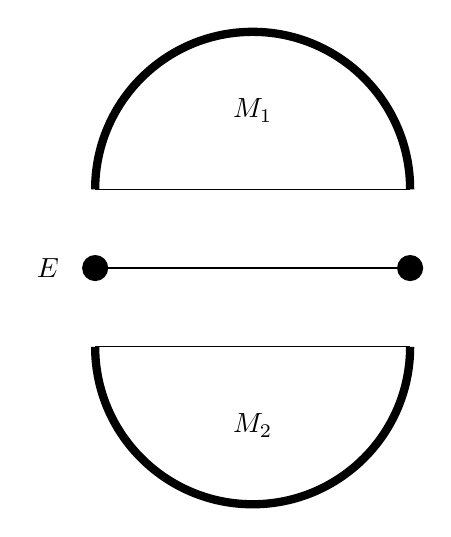
\begin{tikzpicture}[baseline=0]
\coordinate (a) at (0,1);
\coordinate (b) at (4,1);
\draw[marked] (a) arc (180:0:2);
\draw (b) -- (a);
\node at (2,2) {$M_1$};

\draw (0,0) node[fill, circle] {} -- (4,0) node[fill,circle] {};
\node at (-0.6,0) {$E$};

\draw[marked] (0,-1) arc(-180:0:2);
\draw (4,-1) -- (0,-1);
\node at (2,-2) {$M_2$};
\end{tikzpicture}
\qquad \qquad \qquad
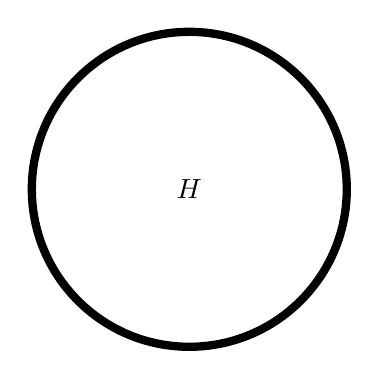
\begin{tikzpicture}[baseline=0]
\draw[marked] (0,0) node {$H$} circle (2);
\end{tikzpicture}
\end{equation*}\caption{The marked hemispheres and marked balls from Lemma \ref{lem:module-boundary}.}
\label{fig:module-boundary}
\end{figure}

Let $\cl\cM(H)\trans E$ denote the image of $\gl_E$.
We will refer to elements of $\cl\cM(H)\trans E$ as ``splittable along $E$" or ``transverse to $E$". 

\noop{ %%%%%%%
\begin{lem}[Module to category restrictions]
{For each marked $k$-hemisphere $H$ there is a restriction map
$\cl\cM(H)\to \cC(H)$.
($\cC(H)$ means apply $\cC$ to the underlying $k$-ball of $H$.)
These maps comprise a natural transformation of functors.}
\end{lem}
}	%%%%%%% end \noop

It follows from the definition of the colimit $\cl\cM(H)$ that
given any (unmarked) $k{-}1$-ball $Y$ in the interior of $H$ there is a restriction map
from a subset $\cl\cM(H)_{\trans{\bdy Y}}$ of $\cl\cM(H)$ to $\cC(Y)$.
Combining this with the boundary map $\cM(B,N) \to \cl\cM(\bd(B,N))$, we also have a restriction
map from a subset $\cM(B,N)_{\trans{\bdy Y}}$ of $\cM(B,N)$ to $\cC(Y)$ whenever $Y$ is in the interior of $\bd B \setmin N$.
This fact will be used below.

\noop{ %%%%
Note that combining the various boundary and restriction maps above
(for both modules and $n$-categories)
we have for each marked $k$-ball $(B, N)$ and each $k{-}1$-ball $Y\sub \bd B \setmin N$
a natural map from a subset of $\cM(B, N)$ to $\cC(Y)$.
This subset $\cM(B,N)\trans{\bdy Y}$ is the subset of morphisms which are appropriately splittable (transverse to the
cutting submanifolds).
This fact will be used below.
} %%%%% end \noop

In our example, the various restriction and gluing maps above come from
restricting and gluing maps into $T$.

We require two sorts of composition (gluing) for modules, corresponding to two ways
of splitting a marked $k$-ball into two (marked or plain) $k$-balls.
(See Figure \ref{zzz3}.)

\begin{figure}[t]
\begin{equation*}
\mathfig{.4}{ncat/zz3}
\end{equation*}
\caption{Module composition (top); $n$-category action (bottom).}
\label{zzz3}
\end{figure}

First, we can compose two module morphisms to get another module morphism.

\begin{module-axiom}[Module composition]
{Let $M = M_1 \cup_Y M_2$, where $M$, $M_1$ and $M_2$ are marked $k$-balls (with $0\le k\le n$)
and $Y = M_1\cap M_2$ is a marked $k{-}1$-ball.
Let $E = \bd Y$, which is a marked $k{-}2$-hemisphere.
Note that each of $M$, $M_1$ and $M_2$ has its boundary split into two marked $k{-}1$-balls by $E$.
We have restriction (domain or range) maps $\cM(M_i)\trans E \to \cM(Y)$.
Let $\cM(M_1) \trans E \times_{\cM(Y)} \cM(M_2) \trans E$ denote the fibered product of these two maps. 
Then (axiom) we have a map
\[
	\gl_Y : \cM(M_1) \trans E \times_{\cM(Y)} \cM(M_2) \trans E \to \cM(M) \trans E
\]
which is natural with respect to the actions of homeomorphisms, and also compatible with restrictions
to the intersection of the boundaries of $M$ and $M_i$.
If $k < n$,
or if $k=n$ and we are in the $A_\infty$ case, 
we require that $\gl_Y$ is injective.
(For $k=n$ in the ordinary (non-$A_\infty$) case, see below.)}
\end{module-axiom}


Second, we can compose an $n$-category morphism with a module morphism to get another
module morphism.
We'll call this the action map to distinguish it from the other kind of composition.

\begin{module-axiom}[$n$-category action]
{Let $M = X \cup_Y M'$, where $M$ and $M'$ are marked $k$-balls ($0\le k\le n$),
$X$ is a plain $k$-ball,
and $Y = X\cap M'$ is a $k{-}1$-ball.
Let $E = \bd Y$, which is a $k{-}2$-sphere.
We have restriction maps $\cM(M') \trans E \to \cC(Y)$ and $\cC(X) \trans E\to \cC(Y)$.
Let $\cC(X)\trans E \times_{\cC(Y)} \cM(M') \trans E$ denote the fibered product of these two maps. 
Then (axiom) we have a map
\[
	\gl_Y :\cC(X)\trans E \times_{\cC(Y)} \cM(M')\trans E \to \cM(M) \trans E
\]
which is natural with respect to the actions of homeomorphisms, and also compatible with restrictions
to the intersection of the boundaries of $X$ and $M'$.
If $k < n$,
or if $k=n$ and we are in the $A_\infty$ case, 
we require that $\gl_Y$ is injective.
(For $k=n$ in the ordinary (non-$A_\infty$) case, see below.)}
\end{module-axiom}

\begin{module-axiom}[Strict associativity]
The composition and action maps above are strictly associative.
Given any decomposition of a large marked ball into smaller marked and unmarked balls
any sequence of pairwise gluings yields (via composition and action maps) the same result.
\end{module-axiom}

Note that the above associativity axiom applies to mixtures of module composition,
action maps and $n$-category composition.
See Figure \ref{zzz1b}.

\begin{figure}[t]
\begin{equation*}
\mathfig{0.49}{ncat/zz0} \mathfig{0.49}{ncat/zz1}
\end{equation*}
\caption{Two examples of mixed associativity}
\label{zzz1b}
\end{figure}


The above three axioms are equivalent to the following axiom,
which we state in slightly vague form.

\xxpar{Module multi-composition:}
{Given any splitting 
\[
	X_1 \sqcup\cdots\sqcup X_p \sqcup M_1\sqcup\cdots\sqcup M_q \to M
\]
of a marked $k$-ball $M$
into small (marked and plain) $k$-balls $M_i$ and $X_j$, there is a 
map from an appropriate subset (like a fibered product) 
of 
\[
	\cC(X_1)\times\cdots\times\cC(X_p) \times \cM(M_1)\times\cdots\times\cM(M_q) 
\]
to $\cM(M)$,
and these various multifold composition maps satisfy an
operad-type strict associativity condition.}

The above operad-like structure is analogous to the swiss cheese operad
\cite{MR1718089}.

\medskip

We can define marked pinched products $\pi:E\to M$ of marked balls analogously to the 
plain ball case.
Note that a marked pinched product can be decomposed into either
two marked pinched products or a plain pinched product and a marked pinched product.
%\nn{should maybe give figure}

\begin{module-axiom}[Product (identity) morphisms]
For each pinched product $\pi:E\to M$, with $M$ a marked $k$-ball and $E$ a marked
$k{+}m$-ball ($m\ge 1$),
there is a map $\pi^*:\cM(M)\to \cM(E)$.
These maps must satisfy the following conditions.
\begin{enumerate}
\item
If $\pi:E\to M$ and $\pi':E'\to M'$ are marked pinched products, and
if $f:M\to M'$ and $\tilde{f}:E \to E'$ are maps such that the diagram
\[ \xymatrix{
	E \ar[r]^{\tilde{f}} \ar[d]_{\pi} & E' \ar[d]^{\pi'} \\
	M \ar[r]^{f} & M'
} \]
commutes, then we have 
\[
	\pi'^*\circ f = \tilde{f}\circ \pi^*.
\]
\item
Product morphisms are compatible with module composition and module action.
Let $\pi:E\to M$, $\pi_1:E_1\to M_1$, and $\pi_2:E_2\to M_2$ 
be pinched products with $E = E_1\cup E_2$.
Let $a\in \cM(M)$, and let $a_i$ denote the restriction of $a$ to $M_i\sub M$.
Then 
\[
	\pi^*(a) = \pi_1^*(a_1)\bullet \pi_2^*(a_2) .
\]
Similarly, if $\rho:D\to X$ is a pinched product of plain balls and
$E = D\cup E_1$, then
\[
	\pi^*(a) = \rho^*(a')\bullet \pi_1^*(a_1),
\]
where $a'$ is the restriction of $a$ to $D$.
\item
Product morphisms are associative.
If $\pi:E\to M$ and $\rho:D\to E$ are marked pinched products then
\[
	\rho^*\circ\pi^* = (\pi\circ\rho)^* .
\]
\item
Product morphisms are compatible with restriction.
If we have a commutative diagram
\[ \xymatrix{
	D \ar@{^(->}[r] \ar[d]_{\rho} & E \ar[d]^{\pi} \\
	Y \ar@{^(->}[r] & M
} \]
such that $\rho$ and $\pi$ are pinched products, then
\[
	\res_D\circ\pi^* = \rho^*\circ\res_Y .
\]
($Y$ could be either a marked or plain ball.)
\end{enumerate}
\end{module-axiom}

As in the $n$-category definition, once we have product morphisms we can define
collar maps $\cM(M)\to \cM(M)$.
Note that there are two cases:
the collar could intersect the marking of the marked ball $M$, in which case
we use a product on a morphism of $\cM$; or the collar could be disjoint from the marking,
in which case we use a product on a morphism of $\cC$.

In our example, elements $a$ of $\cM(M)$ maps to $T$, and $\pi^*(a)$ is the pullback of
$a$ along a map associated to $\pi$.

\medskip

There are two alternatives for the next axiom, according whether we are defining
modules for ordinary $n$-categories or $A_\infty$ $n$-categories.
In the ordinary case we require

\begin{module-axiom}[\textup{\textbf{[ordinary version]}} Extended isotopy invariance in dimension $n$]
{Let $M$ be a marked $n$-ball and $f: M\to M$ be a homeomorphism which restricts
to the identity on $\bd M$ and is isotopic (rel boundary) to the identity.
Then $f$ acts trivially on $\cM(M)$.}
In addition, collar maps act trivially on $\cM(M)$.
\end{module-axiom}

We emphasize that the $\bd M$ above means boundary in the marked $k$-ball sense.
In other words, if $M = (B, N)$ then we require only that isotopies are fixed 
on $\bd B \setmin N$.

For $A_\infty$ modules we require

%\addtocounter{module-axiom}{-1}
\begin{module-axiom}[\textup{\textbf{[$A_\infty$ version]}} Families of homeomorphisms act]
For each marked $n$-ball $M$ and each $c\in \cM(\bd M)$ we have a map of chain complexes
\[
	C_*(\Homeo_\bd(M))\ot \cM(M; c) \to \cM(M; c) .
\]
Here $C_*$ means singular chains and $\Homeo_\bd(M)$ is the space of homeomorphisms of $M$
which fix $\bd M$.
These action maps are required to be associative up to homotopy, as in Theorem \ref{thm:CH-associativity}, 
and also compatible with composition (gluing) in the sense that
a diagram like the one in Theorem \ref{thm:CH} commutes.
\end{module-axiom}

As with the $n$-category version of the above axiom, we should also have families of collar maps act.

\medskip

Note that the above axioms imply that an $n$-category module has the structure
of an $n{-}1$-category.
More specifically, let $J$ be a marked 1-ball, and define $\cE(X)\deq \cM(X\times J)$,
where $X$ is a $k$-ball and in the product $X\times J$ we pinch 
above the non-marked boundary component of $J$.
(More specifically, we collapse $X\times P$ to a single point, where
$P$ is the non-marked boundary component of $J$.)
Then $\cE$ has the structure of an $n{-}1$-category.

All marked $k$-balls are homeomorphic, unless $k = 1$ and our manifolds
are oriented or Spin (but not unoriented or $\text{Pin}_\pm$).
In this case ($k=1$ and oriented or Spin), there are two types
of marked 1-balls, call them left-marked and right-marked,
and hence there are two types of modules, call them right modules and left modules.
In all other cases ($k>1$ or unoriented or $\text{Pin}_\pm$),
there is no left/right module distinction.

\medskip

We now give some examples of modules over ordinary and $A_\infty$ $n$-categories.

\begin{example}[Examples from TQFTs]
\rm
Continuing Example \ref{ex:ncats-from-tqfts}, with $\cF$ a TQFT, $W$ an $n{-}j$-manifold,
and $\cF(W)$ the $j$-category associated to $W$.
Let $Y$ be an $(n{-}j{+}1)$-manifold with $\bd Y = W$.
Define a $\cF(W)$ module $\cF(Y)$ as follows.
If $M = (B, N)$ is a marked $k$-ball with $k<j$ let 
$\cF(Y)(M)\deq \cF((B\times W) \cup (N\times Y))$.
If $M = (B, N)$ is a marked $j$-ball and $c\in \cl{\cF(Y)}(\bd M)$ let
$\cF(Y)(M)\deq A_\cF((B\times W) \cup (N\times Y); c)$.
\end{example}

\begin{example}[Examples from the blob complex] \label{bc-module-example}
\rm
In the previous example, we can instead define
$\cF(Y)(M)\deq \bc_*((B\times W) \cup (N\times Y), c; \cF)$ (when $\dim(M) = n$)
and get a module for the $A_\infty$ $n$-category associated to $\cF$ as in 
Example \ref{ex:blob-complexes-of-balls}.
\end{example}


\begin{example}
\rm
Suppose $S$ is a topological space, with a subspace $T$.
We can define a module $\pi_{\leq n}(S,T)$ so that on each marked $k$-ball $(B,N)$ 
for $k<n$ the set $\pi_{\leq n}(S,T)(B,N)$ consists of all continuous maps of pairs 
$(B,N) \to (S,T)$ and on each marked $n$-ball $(B,N)$ it consists of all 
such maps modulo homotopies fixed on $\bdy B \setminus N$.
This is a module over the fundamental $n$-category $\pi_{\leq n}(S)$ of $S$, from Example \ref{ex:maps-to-a-space}.
\end{example}
Modifications corresponding to Examples \ref{ex:maps-to-a-space-with-a-fiber} and 
\ref{ex:linearized-maps-to-a-space} are also possible, and there is an $A_\infty$ version analogous to 
Example \ref{ex:chains-of-maps-to-a-space} given by taking singular chains.





\subsection{Modules as boundary labels (colimits for decorated manifolds)}
\label{moddecss}

Fix an ordinary $n$-category or $A_\infty$ $n$-category  $\cC$.
Let $W$ be a $k$-manifold ($k\le n$),
let $\{Y_i\}$ be a collection of disjoint codimension 0 submanifolds of $\bd W$,
and let $\cN = (\cN_i)$ be an assignment of a $\cC$ module $\cN_i$ to $Y_i$.

We will define a set $\cC(W, \cN)$ using a colimit construction very similar to 
the one appearing in \S \ref{ss:ncat_fields} above.
(If $k = n$ and our $n$-categories are enriched, then
$\cC(W, \cN)$ will have additional structure; see below.)

Define a permissible decomposition of $W$ to be a map
\[
	\left(\bigsqcup_a X_a\right) \sqcup \left(\bigsqcup_{i,b} M_{ib}\right)  \to W,
\]
where each $X_a$ is a plain $k$-ball disjoint, in $W$, from $\cup Y_i$, and
each $M_{ib}$ is a marked $k$-ball intersecting $Y_i$  (once mapped into $W$),
with $M_{ib}\cap Y_i$ being the marking, which extends to a ball decomposition in the sense of Definition \ref{defn:gluing-decomposition}.
(See Figure \ref{mblabel}.)
\begin{figure}[t]
\begin{equation*}
\mathfig{.4}{ncat/mblabel}
\end{equation*}
\caption{A permissible decomposition of a manifold
whose boundary components are labeled by $\cC$ modules $\{\cN_i\}$.
Marked balls are shown shaded, plain balls are unshaded.}\label{mblabel}
\end{figure}
Given permissible decompositions $x$ and $y$, we say that $x$ is a refinement
of $y$, or write $x \le y$, if each ball of $y$ is a union of balls of $x$.
This defines a partial ordering $\cell(W)$, which we will think of as a category.
(The objects of $\cell(D)$ are permissible decompositions of $W$, and there is a unique
morphism from $x$ to $y$ if and only if $x$ is a refinement of $y$.)

The collection of modules $\cN$ determines 
a functor $\psi_\cN$ from $\cell(W)$ to the category of sets 
(possibly with additional structure if $k=n$).
For a decomposition $x = (X_a, M_{ib})$ in $\cell(W)$, define $\psi_\cN(x)$ to be the subset
\[
	\psi_\cN(x) \sub \left(\prod_a \cC(X_a)\right) \times \left(\prod_{ib} \cN_i(M_{ib})\right)
\]
such that the restrictions to the various pieces of shared boundaries amongst the
$X_a$ and $M_{ib}$ all agree.
(That is, the fibered product over the boundary restriction maps.)
If $x$ is a refinement of $y$, define a map $\psi_\cN(x)\to\psi_\cN(y)$
via the gluing (composition or action) maps from $\cC$ and the $\cN_i$.

We now define the set $\cC(W, \cN)$ to be the colimit of the functor $\psi_\cN$.
(As in \S\ref{ss:ncat-coend}, if $k=n$ we take a colimit in whatever
category we are enriching over, and if additionally we are in the $A_\infty$ case, 
then we use a homotopy colimit.)

\medskip

If $D$ is an $m$-ball, $0\le m \le n-k$, then we can similarly define
$\cC(D\times W, \cN)$, where in this case $\cN_i$ labels the submanifold 
$D\times Y_i \sub \bd(D\times W)$.
It is not hard to see that the assignment $D \mapsto \cC(D\times W, \cN)$
has the structure of an $n{-}k$-category.

\medskip

We will use a simple special case of the above 
construction to define tensor products 
of modules.
Let $\cM_1$ and $\cM_2$ be modules for an $n$-category $\cC$.
(If $k=1$ and our manifolds are oriented, then one should be 
a left module and the other a right module.)
Choose a 1-ball $J$, and label the two boundary points of $J$ by $\cM_1$ and $\cM_2$.
Define the tensor product $\cM_1 \tensor \cM_2$ to be the 
$n{-}1$-category associated as above to $J$ with its boundary labeled by $\cM_1$ and $\cM_2$.
This of course depends (functorially)
on the choice of 1-ball $J$.

We will define a more general self tensor product (categorified coend) below.




\subsection{Morphisms of modules}
\label{ss:module-morphisms}

Modules are collections of functors together with some additional data, so we define morphisms
of modules to be collections of natural transformations which are compatible with this
additional data.

More specifically, let $\cX$ and $\cY$ be $\cC$ modules, i.e.\ collections of functors
$\{\cX_k\}$ and $\{\cY_k\}$, for $0\le k\le n$, from marked $k$-balls to sets 
as in Module Axiom \ref{module-axiom-funct}.
A morphism $g:\cX\to\cY$ is a collection of natural transformations $g_k:\cX_k\to\cY_k$
satisfying:
\begin{itemize}
\item Each $g_k$ commutes with $\bd$.
\item Each $g_k$ commutes with gluing (module composition and $\cC$ action).
\item Each $g_k$ commutes with taking products.
\item In the top dimension $k=n$, $g_n$ preserves whatever additional structure we are enriching over (e.g.\ vector
spaces).
In the $A_\infty$ case (e.g.\ enriching over chain complexes) $g_n$ should live in 
an appropriate derived hom space, as described below.
\end{itemize}

We will be mainly interested in the case $n=1$ and enriched over chain complexes,
since this is the case that's relevant to the generalized Deligne conjecture of \S\ref{sec:deligne}.
So we treat this case in more detail.

First we explain the remark about derived hom above.
Let $L$ be a marked 1-ball and let $\cl{\cX}(L)$ denote the local homotopy colimit construction
associated to $L$ by $\cX$ and $\cC$.
(See \S \ref{ss:ncat_fields} and \S \ref{moddecss}.)
Define $\cl{\cY}(L)$ similarly.
For $K$ an unmarked 1-ball let $\cl{\cC}(K)$ denote the local homotopy colimit
construction associated to $K$ by $\cC$.
Then we have an injective gluing map
\[
	\gl: \cl{\cX}(L) \ot \cl{\cC}(K) \to \cl{\cX}(L\cup K) 
\]
which is also a chain map.
(For simplicity we are suppressing mention of boundary conditions on the unmarked 
boundary components of the 1-balls.)
We define $\hom_\cC(\cX \to \cY)$ to be a collection of (graded linear) natural transformations
$g: \cl{\cX}(L)\to \cl{\cY}(L)$ such that the following diagram commutes for all $L$ and $K$:
\[ \xymatrix{
	\cl{\cX}(L) \ot \cl{\cC}(K) \ar[r]^{\gl} \ar[d]_{g\ot \id} & \cl{\cX}(L\cup K) \ar[d]^{g}\\
	\cl{\cY}(L) \ot \cl{\cC}(K) \ar[r]^{\gl} & \cl{\cY}(L\cup K)
} \]

The usual differential on graded linear maps between chain complexes induces a differential
on $\hom_\cC(\cX \to \cY)$, giving it the structure of a chain complex.

Let $\cZ$ be another $\cC$ module.
We define a chain map
\[
	a: \hom_\cC(\cX \to \cY) \ot (\cX \ot_\cC \cZ) \to \cY \ot_\cC \cZ
\]
as follows.
Recall that the tensor product $\cX \ot_\cC \cZ$  depends on a choice of interval $J$, labeled
by $\cX$ on one boundary component and $\cZ$ on the other.
Because we are using the {\it local} homotopy colimit, any generator
$D\ot x\ot \bar{c}\ot z$ of $\cX \ot_\cC \cZ$ can be written (perhaps non-uniquely) as a gluing
$(D'\ot x \ot \bar{c}') \bullet (D''\ot \bar{c}''\ot z)$, for some decomposition $J = L'\cup L''$
and with $D'\ot x \ot \bar{c}'$ a generator of $\cl{\cX}(L')$ and 
$D''\ot \bar{c}''\ot z$ a generator of $\cl{\cZ}(L'')$.
(Such a splitting exists because the blob diagram $D$ can be split into left and right halves, 
since no blob can include both the leftmost and rightmost intervals in the underlying decomposition.
This step would fail if we were using the usual hocolimit instead of the local hocolimit.)
We now define
\[
	a: g\ot (D\ot x\ot \bar{c}\ot z) \mapsto g(D'\ot x \ot \bar{c}')\bullet (D''\ot \bar{c}''\ot z) .
\]
This does not depend on the choice of splitting $D = D'\bullet D''$ because $g$ commutes with gluing.




\subsection{The \texorpdfstring{$n{+}1$}{n+1}-category of sphere modules}
\label{ssec:spherecat}

In this subsection we define $n{+}1$-categories $\cS$ of ``sphere modules".
The objects are $n$-categories, the $k$-morphisms are $k{-}1$-sphere modules for $1\le k \le n$,
and the $n{+}1$-morphisms are intertwiners.
With future applications in mind, we treat simultaneously the big category
of all $n$-categories and all sphere modules and also subcategories thereof.
When $n=1$ this is closely related to familiar $2$-categories consisting of 
algebras, bimodules and intertwiners (or a subcategory of that).
The sphere module $n{+}1$-category is a natural generalization of the 
algebra-bimodule-intertwiner 2-category to higher dimensions.

Another possible name for this $n{+}1$-category is the $n{+}1$-category of defects.
The $n$-categories are thought of as representing field theories, and the 
$0$-sphere modules are codimension 1 defects between adjacent theories.
In general, $m$-sphere modules are codimension $m{+}1$ defects;
the link of such a defect is an $m$-sphere decorated with defects of smaller codimension.

\medskip

While it is appropriate to call an $S^0$ module a bimodule,
this is much less true for higher dimensional spheres, 
so we prefer the term ``sphere module" for the general case.

For simplicity, we will assume that $n$-categories are enriched over $\c$-vector spaces.

The $0$- through $n$-dimensional parts of $\cS$ are various sorts of modules, and we describe
these first.
The $n{+}1$-dimensional part of $\cS$ consists of intertwiners
of  $1$-category modules associated to decorated $n$-balls.
We will see below that in order for these $n{+}1$-morphisms to satisfy all of
the axioms of an $n{+}1$-category (in particular, duality requirements), we will have to assume
that our $n$-categories and modules have non-degenerate inner products.
(In other words, we need to assume some extra duality on the $n$-categories and modules.)

\medskip

Our first task is to define an $n$-category $m$-sphere module, for $0\le m \le n-1$.
These will be defined in terms of certain classes of marked balls, very similarly
to the definition of $n$-category modules above.
(This, in turn, is very similar to our definition of $n$-category.)
Because of this similarity, we only sketch the definitions below.

We start with $0$-sphere modules, which also could reasonably be called (categorified) bimodules.
(For $n=1$ they are precisely bimodules in the usual, uncategorified sense.)
We prefer the more awkward term ``0-sphere module" to emphasize the analogy
with the higher sphere modules defined below.

Define a $0$-marked $k$-ball, $1\le k \le n$, to be a pair  $(X, M)$ homeomorphic to the standard
$(B^k, B^{k-1})$.
See Figure \ref{feb21a}.
Another way to say this is that $(X, M)$ is homeomorphic to $B^{k-1}\times([-1,1], \{0\})$.

\begin{figure}[t]
$$\tikz[baseline,line width=2pt]{\draw[blue] (-2,0)--(2,0); \fill[red] (0,0) circle (0.1);} \qquad \qquad \tikz[baseline,line width=2pt]{\draw[blue][fill=blue!30!white] (0,0) circle (2 and 1); \draw[red] (0,1)--(0,-1);}$$
\caption{0-marked 1-ball and 0-marked 2-ball}
\label{feb21a}
\end{figure}

The $0$-marked balls can be cut into smaller balls in various ways.
We only consider those decompositions in which the smaller balls are either
$0$-marked (i.e. intersect the $0$-marking of the large ball in a disc) 
or plain (don't intersect the $0$-marking of the large ball).
We can also take the boundary of a $0$-marked ball, which is a $0$-marked sphere.

Fix $n$-categories $\cA$ and $\cB$.
These will label the two halves of a $0$-marked $k$-ball.

An $n$-category $0$-sphere module $\cM$ over the $n$-categories $\cA$ and $\cB$ is 
a collection of functors $\cM_k$ from the category
of $0$-marked $k$-balls, $1\le k \le n$,
(with the two halves labeled by $\cA$ and $\cB$) to the category of sets.
If $k=n$ these sets should be enriched to the extent $\cA$ and $\cB$ are.
Given a decomposition of a $0$-marked $k$-ball $X$ into smaller balls $X_i$, we have
morphism sets $\cA_k(X_i)$ (if $X_i$ lies on the $\cA$-labeled side)
or $\cB_k(X_i)$ (if $X_i$ lies on the $\cB$-labeled side)
or $\cM_k(X_i)$ (if $X_i$ intersects the marking and is therefore a smaller 0-marked ball).
Corresponding to this decomposition we have a composition (or ``gluing") map
from the product (fibered over the boundary data) of these various sets into $\cM_k(X)$.

\medskip

Part of the structure of an $n$-category 0-sphere module $\cM$  is captured by saying it is
a collection $\cD^{ab}$ of $n{-}1$-categories, indexed by pairs $(a, b)$ of objects (0-morphisms)
of $\cA$ and $\cB$.
Let $J$ be some standard 0-marked 1-ball (i.e.\ an interval with a marked point in its interior).
Given a $j$-ball $X$, $0\le j\le n-1$, we define
\[
	\cD(X) \deq \cM(X\times J) .
\]
The product is pinched over the boundary of $J$.
The set $\cD$ breaks into ``blocks" according to the restrictions to the pinched points of $X\times J$
(see Figure \ref{feb21b}).
These restrictions are 0-morphisms $(a, b)$ of $\cA$ and $\cB$.

\begin{figure}[t] \centering
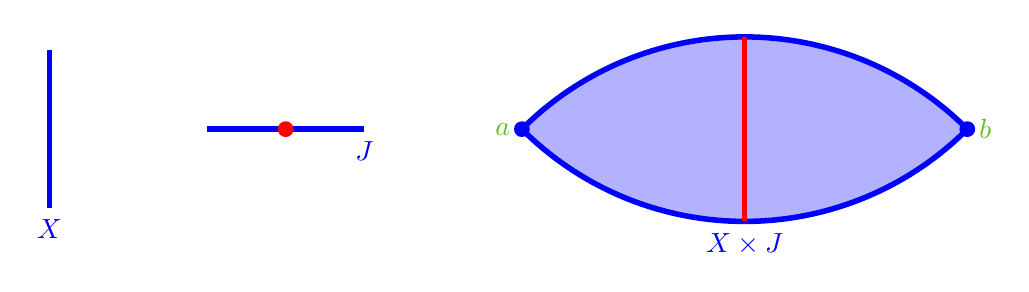
\begin{tikzpicture}[blue,line width=2pt]
\draw (0,1) -- (0,-1) node[below] {$X$};

\draw (2,0) -- (4,0) node[below] {$J$};
\fill[red] (3,0) circle (0.1);

\draw[fill=blue!30!white] (6,0) node(a) {} arc (135:90:4) node(top) {} arc (90:45:4) node(b) {} arc (-45:-90:4) node(bottom) {} arc(-90:-135:4);
\draw[red] (top.center) -- (bottom.center);
\fill (a) circle (0.1) node[left] {\color{green!50!brown} $a$};
\fill (b) circle (0.1) node[right] {\color{green!50!brown} $b$};

\path (bottom) node[below]{$X \times J$};

\end{tikzpicture}
\caption{The pinched product $X\times J$}
\label{feb21b}
\end{figure}

More generally, consider an interval with interior marked points, and with the complements
of these points labeled by $n$-categories $\cA_i$ ($0\le i\le l$) and the marked points labeled
by $\cA_i$-$\cA_{i+1}$ 0-sphere modules $\cM_i$.
(See Figure \ref{feb21c}.)
To this data we can apply the coend construction as in \S\ref{moddecss} above
to obtain an $\cA_0$-$\cA_l$ $0$-sphere module and, forgetfully, an $n{-}1$-category.
This amounts to a definition of taking tensor products of $0$-sphere modules over $n$-categories.

\begin{figure}[t] \centering
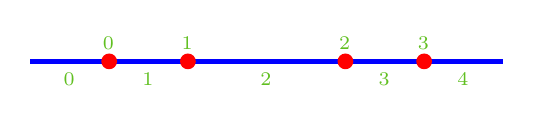
\begin{tikzpicture}[baseline,line width = 2pt]
\draw[blue] (0,0) -- (6,0);
\foreach \x/\n in {0.5/0,1.5/1,3/2,4.5/3,5.5/4} {
	\path (\x,0)  node[below] {\color{green!50!brown}$\cA_{\n}$};
}
\foreach \x/\n in {1/0,2/1,4/2,5/3} {
	\fill[red] (\x,0) circle (0.1) node[above] {\color{green!50!brown}$\cM_{\n}$};
}
\end{tikzpicture}
\qquad
\qquad
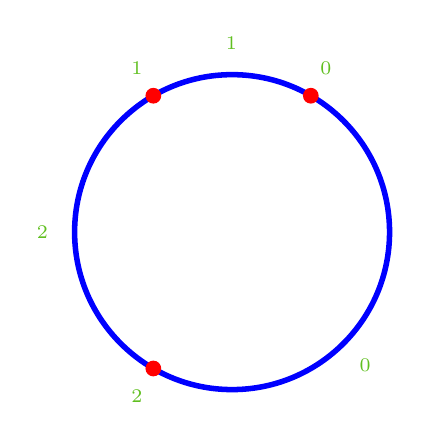
\begin{tikzpicture}[baseline,line width = 2pt]
\draw[blue] (0,0) circle (2);
\foreach \q/\n in {-45/0,90/1,180/2} {
	\path (\q:2.4)  node {\color{green!50!brown}$\cA_{\n}$};
}
\foreach \q/\n in {60/0,120/1,-120/2} {
	\fill[red] (\q:2) circle (0.1);
	\path (\q:2.4) node {\color{green!50!brown}$\cM_{\n}$};
}
\end{tikzpicture}
\caption{Marked and labeled 1-manifolds}
\label{feb21c}
\end{figure}

We could also similarly mark and label a circle, obtaining an $n{-}1$-category
associated to the marked and labeled circle.
(See Figure \ref{feb21c}.)
If the circle is divided into two intervals, we can think of this $n{-}1$-category
as the 2-sided tensor product of the two 0-sphere modules associated to the two intervals.

\medskip

Next we define $n$-category 1-sphere modules.
These are just representations of (modules for) $n{-}1$-categories associated to marked and labeled 
circles (1-spheres) which we just introduced.

Equivalently, we can define 1-sphere modules in terms of 1-marked $k$-balls, $2\le k\le n$.
Fix a marked (and labeled) circle $S$.
Let $C(S)$ denote the cone of $S$, a marked 2-ball (Figure \ref{feb21d}).
%\nn{I need to make up my mind whether marked things are always labeled too.
%For the time being, let's say they are.}
A 1-marked $k$-ball is anything homeomorphic to $B^j \times C(S)$, $0\le j\le n-2$, 
where $B^j$ is the standard $j$-ball.
A 1-marked $k$-ball can be decomposed in various ways into smaller balls, which are either 
(a) smaller 1-marked $k$-balls, (b) 0-marked $k$-balls, or (c) plain $k$-balls.
(See Figure \ref{subdividing1marked}.)
We now proceed as in the above module definitions.

\begin{figure}[t] \centering
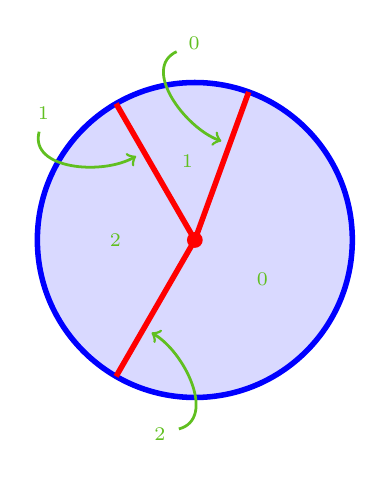
\begin{tikzpicture}[baseline,line width = 2pt]
\draw[blue][fill=blue!15!white] (0,0) circle (2);
\fill[red] (0,0) circle (0.1);
\foreach \qm/\qa/\n in {70/-30/0, 120/95/1, -120/180/2} {
	\draw[red] (0,0) -- (\qm:2);
	\path (\qa:1) node {\color{green!50!brown} $\cA_\n$};
	\path (\qm+20:2.5) node(M\n) {\color{green!50!brown} $\cM_\n$};
	\draw[line width=1pt, green!50!brown, ->] (M\n.\qm+135) to[out=\qm+135,in=\qm+90] (\qm+5:1.3);
}
\end{tikzpicture}
\caption{Cone on a marked circle, the prototypical 1-marked ball}
\label{feb21d}
\end{figure}

\begin{figure}[t] \centering
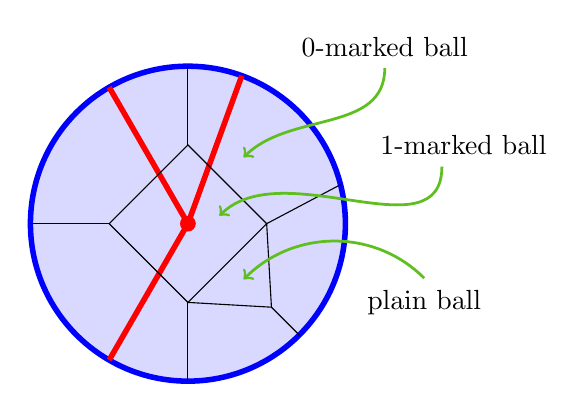
\begin{tikzpicture}[baseline,line width = 2pt]
\draw[blue][fill=blue!15!white] (0,0) circle (2);
\fill[red] (0,0) circle (0.1);
\foreach \qm/\qa/\n in {70/-30/0, 120/95/1, -120/180/2} {
	\draw[red] (0,0) -- (\qm:2);
%	\path (\qa:1) node {\color{green!50!brown} $\cA_\n$};
%	\path (\qm+20:2.5) node(M\n) {\color{green!50!brown} $\cM_\n$};
%	\draw[line width=1pt, green!50!brown, ->] (M\n.\qm+135) to[out=\qm+135,in=\qm+90] (\qm+5:1.3);
}


\begin{scope}[black, thin]
\clip (0,0) circle (2);
\draw (0:1) -- (90:1) -- (180:1) -- (270:1) -- cycle;
\draw (90:1) -- (90:2.1);
\draw (180:1) -- (180:2.1);
\draw (270:1) -- (270:2.1);
\draw (0:1) -- (15:2.1);
\draw (0:1) -- (315:1.5) -- (270:1);
\draw (315:1.5) -- (315:2.1);
\end{scope}

\node(0marked) at (2.5,2.25) {$0$-marked ball};
\node(1marked) at (3.5,1) {$1$-marked ball};
\node(plain) at (3,-1) {plain ball};
\draw[line width=1pt, green!50!brown, ->] (0marked.270) to[out=270,in=45] (50:1.1);
\draw[line width=1pt, green!50!brown, ->] (1marked.225) to[out=270,in=45] (0.4,0.1);
\draw[line width=1pt, green!50!brown, ->] (plain.90) to[out=135,in=45] (-45:1);

\end{tikzpicture}
\caption{Subdividing a $1$-marked ball into plain, $0$-marked and $1$-marked balls.}
\label{subdividing1marked}
\end{figure}

A $n$-category 1-sphere module is, among other things, an $n{-}2$-category $\cD$ with
\[
	\cD(X) \deq \cM(X\times C(S)) .
\]
The product is pinched over the boundary of $C(S)$.
$\cD$ breaks into ``blocks" according to the restriction to the 
image of $\bd C(S) = S$ in $X\times C(S)$.

More generally, consider a 2-manifold $Y$ 
(e.g.\ 2-ball or 2-sphere) marked by an embedded 1-complex $K$.
The components of $Y\setminus K$ are labeled by $n$-categories, 
the edges of $K$ are labeled by 0-sphere modules, 
and the 0-cells of $K$ are labeled by 1-sphere modules.
We can now apply the coend construction and obtain an $n{-}2$-category.
If $Y$ has boundary then this $n{-}2$-category is a module for the $n{-}1$-category
associated to the (marked, labeled) boundary of $Y$.
In particular, if $\bd Y$ is a 1-sphere then we get a 1-sphere module as defined above.

\medskip

It should now be clear how to define $n$-category $m$-sphere modules for $0\le m \le n-1$.
For example, there is an $n{-}2$-category associated to a marked, labeled 2-sphere,
and a 2-sphere module is a representation of such an $n{-}2$-category.

\medskip

We can now define the $n$-or-less-dimensional part of our $n{+}1$-category $\cS$.
Choose some collection of $n$-categories, then choose some collections of 0-sphere modules between
these $n$-categories, then choose some collection of 1-sphere modules for the various
possible marked 1-spheres labeled by the $n$-categories and 0-sphere modules, and so on.
Let $L_i$ denote the collection of $i{-}1$-sphere modules we have chosen.
(For convenience, we declare a $(-1)$-sphere module to be an $n$-category.)
There is a wide range of possibilities.
The set $L_0$ could contain infinitely many $n$-categories or just one.
For each pair of $n$-categories in $L_0$, $L_1$ could contain no 0-sphere modules at all or 
it could contain several.
The only requirement is that each $k$-sphere module be a module for a $k$-sphere $n{-}k$-category
constructed out of labels taken from $L_j$ for $j<k$.

We remind the reader again that $\cS = \cS_{\{L_i\}, \{z_Y\}}$ depends on 
the choice of $L_i$ above as well as the choice of 
families of inner products below.

We now define $\cS(X)$, for $X$ a ball of dimension at most $n$, to be the set of all 
cell-complexes $K$ embedded in $X$, with the codimension-$j$ parts of $(X, K)$ labeled
by elements of $L_j$.
As described above, we can think of each decorated $k$-ball as defining a $k{-}1$-sphere module
for the $n{-}k{+}1$-category associated to its decorated boundary.
Thus the $k$-morphisms of $\cS$ (for $k\le n$) can be thought 
of as $n$-category $k{-}1$-sphere modules 
(generalizations of bimodules).
On the other hand, we can equally well think of the $k$-morphisms as decorations on $k$-balls, 
and from this point of view it is clear that they satisfy all of the axioms of an
$n{+}1$-category.
(All of the axioms for the less-than-$n{+}1$-dimensional part of an $n{+}1$-category, that is.)

\medskip

Next we define the $n{+}1$-morphisms of $\cS$.
The construction of the 0- through $n$-morphisms was easy and tautological, but the 
$n{+}1$-morphisms will require some effort and combinatorial topology, as well as additional
duality assumptions on the lower morphisms. 
These are required because we define the spaces of $n{+}1$-morphisms by 
making arbitrary choices of incoming and outgoing boundaries for each $n$-ball. 
The additional duality assumptions are needed to prove independence of our definition from these choices.

Let $X$ be an $n{+}1$-ball, and let $c$ be a decoration of its boundary
by a cell complex labeled by 0- through $n$-morphisms, as above.
Choose an $n{-}1$-sphere $E\sub \bd X$, transverse to $c$, which divides
$\bd X$ into ``incoming" and ``outgoing" boundary $\bd_-X$ and $\bd_+X$.
Let $E_c$ denote $E$ decorated by the restriction of $c$ to $E$.
Recall from above the associated 1-category $\cS(E_c)$.
We can also have $\cS(E_c)$ modules $\cS(\bd_-X_c)$ and $\cS(\bd_+X_c)$.
Define
\[
	\cS(X; c; E) \deq \hom_{\cS(E_c)}(\cS(\bd_-X_c), \cS(\bd_+X_c)) .
\]

We will show that if the sphere modules are equipped with a ``compatible family of 
non-degenerate inner products", then there is a coherent family of isomorphisms
$\cS(X; c; E) \cong \cS(X; c; E')$ for all pairs of choices $E$ and $E'$.
This will allow us to define $\cS(X; c)$ independently of the choice of $E$.

First we must define ``inner product", ``non-degenerate" and ``compatible".
Let $Y$ be a decorated $n$-ball, and $\ol{Y}$ its mirror image.
(We assume we are working in the unoriented category.)
Let $Y\cup\ol{Y}$ denote the decorated $n$-sphere obtained by gluing $Y$ and $\ol{Y}$
along their common boundary.
An {\it inner product} on $\cS(Y)$ is a dual vector
\[
	z_Y : \cS(Y\cup\ol{Y}) \to \c.
\]
We will also use the notation
\[
	\langle a, b\rangle \deq z_Y(a\bullet b) \in \c .
\]
An inner product induces a linear map
\begin{eqnarray*}
	\varphi: \cS(Y) &\to& \cS(Y)^* \\
	a &\mapsto& \langle a, \cdot \rangle
\end{eqnarray*}
which satisfies, for all morphisms $e$ of $\cS(\bd Y)$,
\[
	\varphi(ae)(b) = \langle ae, b \rangle = z_Y(a\bullet e\bullet b) = 
			\langle a, eb \rangle = \varphi(a)(eb) .
\]
In other words, $\varphi$ is a map of $\cS(\bd Y)$ modules.
An inner product is {\it non-degenerate} if $\varphi$ is an isomorphism.
This implies that $\cS(Y; c)$ is finite dimensional for all boundary conditions $c$.
(One can think of these inner products as giving some duality in dimension $n{+}1$;
heretofore we have only assumed duality in dimensions 0 through $n$.)

Next we define compatibility.
Let $Y = Y_1\cup Y_2$ with $D = Y_1\cap Y_2$.
Let $X_1$ and $X_2$ be the two components of $Y\times I$ cut along
$D\times I$, in both cases using the pinched product.
(Here we are overloading notation and letting $D$ denote both a decorated and an undecorated
manifold.)
We have $\bd X_i = Y_i \cup \ol{Y}_i \cup (D\times I)$
(see Figure \ref{jun23a}).
\begin{figure}[t]
\begin{equation*}
\mathfig{.6}{ncat/YxI-sliced}
\end{equation*}
\caption{$Y\times I$ sliced open}
\label{jun23a}
\end{figure}
Given $a_i\in \cS(Y_i)$, $b_i\in \cS(\ol{Y}_i)$ and $v\in\cS(D\times I)$
which agree on their boundaries, we can evaluate
\[
	z_{Y_i}(a_i\bullet b_i\bullet v) \in \c .
\]
(This requires a choice of homeomorphism $Y_i \cup \ol{Y}_i \cup (D\times I) \cong
Y_i \cup \ol{Y}_i$, but the value of $z_{Y_i}$ is independent of this choice.)
We can think of $z_{Y_i}$ as giving a function
\[
	\psi_i : \cS(Y_i) \ot \cS(\ol{Y}_i) \to \cS(D\times I)^* 
					\stackrel{\varphi\inv}{\longrightarrow} \cS(D\times I) .
\]
We can now finally define a family of inner products to be {\it compatible} if
for all decompositions $Y = Y_1\cup Y_2$ as above and all $a_i\in \cS(Y_i)$, $b_i\in \cS(\ol{Y}_i)$
we have
\[
	z_Y(a_1\bullet a_2\bullet b_1\bullet b_2) = 
				z_{D\times I}(\psi_1(a_1\ot b_1)\bullet \psi_2(a_2\ot b_2)) .
\]
In other words, the inner product on $Y$ is determined by the inner products on
$Y_1$, $Y_2$ and $D\times I$.

Now we show how to unambiguously identify $\cS(X; c; E)$ and $\cS(X; c; E')$ for any
two choices of $E$ and $E'$.
Consider first the case where $\bd X$ is decomposed as three $n$-balls $A$, $B$ and $C$,
with $E = \bd(A\cup B)$ and $E' = \bd A$.
We must provide an isomorphism between $\cS(X; c; E) = \hom(\cS(C), \cS(A\cup B))$
and $\cS(X; c; E') = \hom(\cS(C\cup \ol{B}), \cS(A))$.
Let $D = B\cap A$.
Then as above we can construct a map
\[
	\psi: \cS(B)\ot\cS(\ol{B}) \to \cS(D\times I) .
\]
Given $f\in \hom(\cS(C), \cS(A\cup B))$ we define $f'\in \hom(\cS(C\cup \ol{B}), \cS(A))$
to be the composition
\[
	\cS(C\cup \ol{B}) \stackrel{f\ot\id}{\longrightarrow}
		\cS(A\cup B\cup \ol{B})  \stackrel{\id\ot\psi}{\longrightarrow}
			\cS(A\cup(D\times I)) \stackrel{\cong}{\longrightarrow} \cS(A) .
\]
(See Figure \ref{jun23b}.)
\begin{figure}[t]
$$
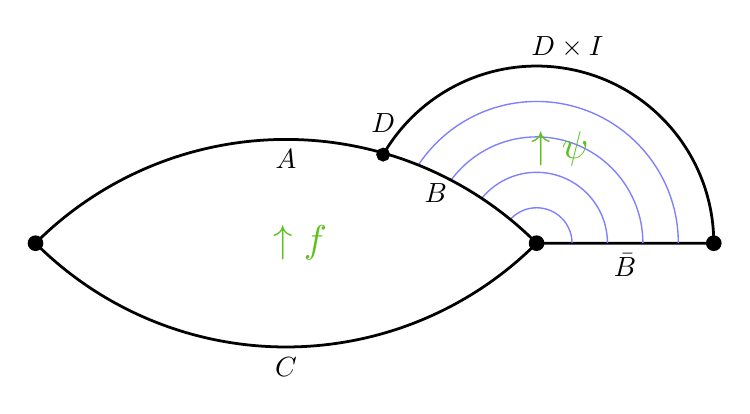
\begin{tikzpicture}[baseline,line width = 1pt,x=1.5cm,y=1.5cm]
\draw (0,0) node(R) {}
	-- (0.75,0) node[below] {$\bar{B}$}
	--(1.5,0)  node[circle,fill=black,inner sep=2pt] {}
	arc (0:80:1.5) node[above] {$D \times I$}
	arc (80:180:1.5);
\foreach \r in {0.3, 0.6, 0.9, 1.2} {
	\draw[blue!50, line width = 0.5pt] (\r,0) arc (0:180:\r);
}
\draw[fill=white]
	(R) node[circle,fill=black,inner sep=2pt] {}
	arc (45:65:3) node[below] {$B$}
	arc (65:90:3) node[below] {$A$}
	arc (90:135:3) node[circle,fill=black,inner sep=2pt] {}
	arc (-135:-90:3) node[below] {$C$}
	arc (-90:-45:3);
\draw[fill]  (150:1.5) circle (2pt) node[above=4pt] {$D$};
\node[green!50!brown] at (-2,0) {\scalebox{1.4}{$\uparrow f$}};
\node[green!50!brown] at (0.2,0.8) {\scalebox{1.4}{$\uparrow \psi$}};
\end{tikzpicture}
$$
\caption{Moving $B$ from top to bottom}
\label{jun23b}
\end{figure}
Let $D' = B\cap C$.
Using the inner products there is an adjoint map
\[
	\psi^\dagger: \cS(D'\times I) \to \cS(\ol{B})\ot\cS(B) .
\]
Given $f'\in \hom(\cS(C\cup \ol{B}), \cS(A))$ we define $f\in \hom(\cS(C), \cS(A\cup B))$
to be the composition
\[
	\cS(C) \stackrel{\cong}{\longrightarrow}
		\cS(C\cup(D'\times I)) \stackrel{\id\ot\psi^\dagger}{\longrightarrow}
			\cS(C\cup \ol{B}\cup B)   \stackrel{f'\ot\id}{\longrightarrow}
				\cS(A\cup B) .
\]
(See Figure \ref{jun23c}.)
\begin{figure}[t]
\begin{equation*}
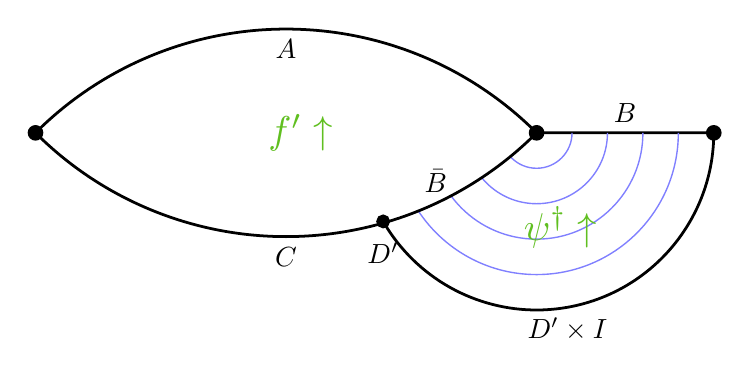
\begin{tikzpicture}[baseline,line width = 1pt,x=1.5cm,y=-1.5cm]
\draw (0,0) node(R) {}
	-- (0.75,0) node[above] {$B$}
	--(1.5,0)  node[circle,fill=black,inner sep=2pt] {}
	arc (0:80:1.5) node[below] {$D' \times I$}
	arc (80:180:1.5);
\foreach \r in {0.3, 0.6, 0.9, 1.2} {
	\draw[blue!50, line width = 0.5pt] (\r,0) arc (0:180:\r);
}
\draw[fill=white]
	(R) node[circle,fill=black,inner sep=2pt] {}
	arc (45:65:3) node[above] {$\bar{B}$}
	arc (65:90:3) node[below] {$C$}
	arc (90:135:3) node[circle,fill=black,inner sep=2pt] {}
	arc (-135:-90:3) node[below] {$A$}
	arc (-90:-45:3);
\draw[fill]  (150:1.5) circle (2pt) node[below=4pt] {$D'$};
\node[green!50!brown] at (-2,0) {\scalebox{1.4}{$f'\uparrow $}};
\node[green!50!brown] at (0.2,0.8) {\scalebox{1.4}{$\psi^\dagger \uparrow $}};
\end{tikzpicture}
\end{equation*}
\caption{Moving $B$ from bottom to top}
\label{jun23c}
\end{figure}
It is not hard too show that the above two maps are mutually inverse.

\begin{lem} \label{equator-lemma}
Any two choices of $E$ and $E'$ are related by a series of modifications as above.
\end{lem}

\begin{proof}
(Sketch)
$E$ and $E'$ are isotopic, and any isotopy is 
homotopic to a composition of small isotopies which are either
(a) supported away from $E$, or (b) modify $E$ in the simple manner described above.
\end{proof}

It follows from the lemma that we can construct an isomorphism
between $\cS(X; c; E)$ and $\cS(X; c; E')$ for any pair $E$, $E'$.
This construction involves a choice of simple ``moves" (as above) to transform
$E$ to $E'$.
We must now show that the isomorphism does not depend on this choice.
We will show below that it suffices to check two ``movie moves".

The first movie move is to push $E$ across an $n$-ball $B$ as above, then push it back.
The result is equivalent to doing nothing.
As we remarked above, the isomorphisms corresponding to these two pushes are mutually
inverse, so we have invariance under this movie move.

The second movie move replaces two successive pushes in the same direction,
across $B_1$ and $B_2$, say, with a single push across $B_1\cup B_2$.
(See Figure \ref{jun23d}.)
\begin{figure}[t]
\begin{tikzpicture}
\node(L) {
\scalebox{0.5}{
\begin{tikzpicture}[baseline,line width = 1pt,x=1.5cm,y=1.5cm]
\draw[red] (0.75,0) -- +(2,0);
\draw[red] (0,0) node(R) {}
	-- (0.75,0) node[below] {}
	--(1.5,0)  node[circle,fill=black,inner sep=2pt] {};
\draw[fill]  (150:1.5) circle (2pt) node[above=4pt] {};
\draw (1.5,0) arc (0:149:1.5);
\draw[red]
	(R) node[circle,fill=black,inner sep=2pt] {}
	arc (-45:-135:3) node[circle,fill=black,inner sep=2pt] {};
\draw[red] (-5.5,0) -- (-4.2,0);
\draw (R) arc (45:75:3);
\draw (150:1.5) arc (74:135:3);
\node at (-2,0) {\scalebox{2.0}{$B_1$}};
\node at (0.2,0.8) {\scalebox{2.0}{$B_2$}};
\node at (-4,1.2) {\scalebox{2.0}{$A$}};
\node at (-4,-1.2) {\scalebox{2.0}{$C$}};
\node[red] at (2.53,0.35) {\scalebox{2.0}{$E$}};
\end{tikzpicture}
}
};
\node(M) at (5,4) {
\scalebox{0.5}{
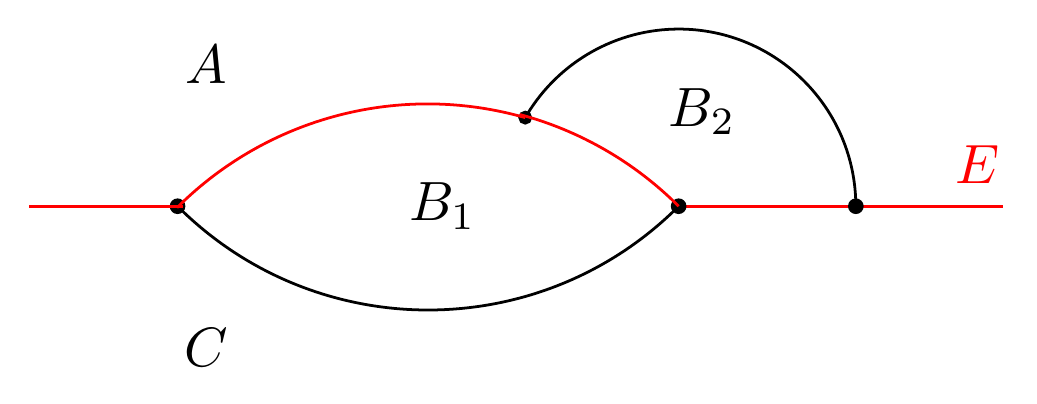
\begin{tikzpicture}[baseline,line width = 1pt,x=1.5cm,y=1.5cm]
\draw[red] (0.75,0) -- +(2,0);
\draw[red] (0,0) node(R) {}
	-- (0.75,0) node[below] {}
	--(1.5,0)  node[circle,fill=black,inner sep=2pt] {};
\draw[fill]  (150:1.5) circle (2pt) node[above=4pt] {};
\draw(1.5,0) arc (0:149:1.5);
\draw
	(R) node[circle,fill=black,inner sep=2pt] {}
	arc (-45:-135:3) node[circle,fill=black,inner sep=2pt] {};
\draw[red] (-5.5,0) -- (-4.2,0);
\draw[red] (R) arc (45:75:3);
\draw[red] (150:1.5) arc (74:135:3);
\node at (-2,0) {\scalebox{2.0}{$B_1$}};
\node at (0.2,0.8) {\scalebox{2.0}{$B_2$}};
\node at (-4,1.2) {\scalebox{2.0}{$A$}};
\node at (-4,-1.2) {\scalebox{2.0}{$C$}};
\node[red] at (2.53,0.35) {\scalebox{2.0}{$E$}};
\end{tikzpicture}
}
};
\node(R) at (10,0) {
\scalebox{0.5}{
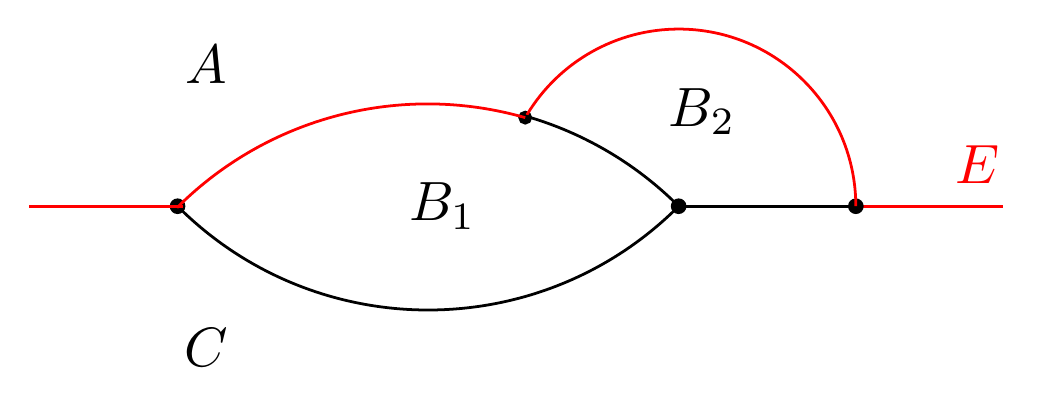
\begin{tikzpicture}[baseline,line width = 1pt,x=1.5cm,y=1.5cm]
\draw[red] (0.75,0) -- +(2,0);
\draw (0,0) node(R) {}
	-- (0.75,0) node[below] {}
	--(1.5,0)  node[circle,fill=black,inner sep=2pt] {};
\draw[fill]  (150:1.5) circle (2pt) node[above=4pt] {};
\draw[red] (1.5,0) arc (0:149:1.5);
\draw
	(R) node[circle,fill=black,inner sep=2pt] {}
	arc (-45:-135:3) node[circle,fill=black,inner sep=2pt] {};
\draw[red] (-5.5,0) -- (-4.2,0);
\draw (R) arc (45:75:3);
\draw[red] (150:1.5) arc (74:135:3);
\node at (-2,0) {\scalebox{2.0}{$B_1$}};
\node at (0.2,0.8) {\scalebox{2.0}{$B_2$}};
\node at (-4,1.2) {\scalebox{2.0}{$A$}};
\node at (-4,-1.2) {\scalebox{2.0}{$C$}};
\node[red] at (2.53,0.35) {\scalebox{2.0}{$E$}};
\end{tikzpicture}
}
};
\draw[->] (L) to[out=90,in=225] node[sloped, above] {push $B_1$} (M);
\draw[->] (M)  to[out=-45,in=90] node[sloped, above] {push $B_2$} (R);
\draw[->] (L) to[out=-35,in=-145] node[sloped, below] {push $B_1 \cup B_2$} (R);
\end{tikzpicture}
\caption{A movie move}
\label{jun23d}
\end{figure}
Invariance under this movie move follows from the compatibility of the inner
product for $B_1\cup B_2$ with the inner products for $B_1$ and $B_2$.

%The third movie move could be called ``locality" or ``disjoint commutativity".
%\nn{...}

If $n\ge 2$, these two movie moves suffice:

\begin{lem}
Assume $n\ge 2$ and fix $E$ and $E'$ as above.
Then any two sequences of elementary moves connecting $E$ to $E'$
are related by a sequence of the two movie moves defined above.
\end{lem}

\begin{proof}
(Sketch)
Consider a two parameter family of diffeomorphisms (one parameter family of isotopies) 
of $\bd X$.
Up to homotopy,
such a family is homotopic to a family which can be decomposed 
into small families which are either
(a) supported away from $E$, 
(b) have boundaries corresponding to the two movie moves above.
Finally, observe that the space of $E$'s is simply connected.
(This fails for $n=1$.)
\end{proof}

For $n=1$ we have to check an additional ``global" relation corresponding to 
rotating the 0-sphere $E$ around the 1-sphere $\bd X$.
But if $n=1$, then we are in the case of ordinary algebroids and bimodules,
and this is just the well-known ``Frobenius reciprocity" result for bimodules \cite{MR1424954}.

\medskip

We have now defined $\cS(X; c)$ for any $n{+}1$-ball $X$ with boundary decoration $c$.
We must also define, for any homeomorphism $X\to X'$, an action $f: \cS(X; c) \to \cS(X', f(c))$.
Choosing an equator $E\sub \bd X$ we have 
\[
	\cS(X; c) \cong \cS(X; c; E) \deq \hom_{\cS(E_c)}(\cS(\bd_-X_c), \cS(\bd_+X_c)) .
\]
We define $f: \cS(X; c) \to \cS(X', f(c))$ to be the tautological map
\[
	f: \cS(X; c; E) \to \cS(X'; f(c); f(E)) .
\]
It is easy to show that this is independent of the choice of $E$.
Note also that this map depends only on the restriction of $f$ to $\bd X$.
In particular, if $F: X\to X$ is the identity on $\bd X$ then $f$ acts trivially, as required by
Axiom \ref{axiom:extended-isotopies}.

We define product $n{+}1$-morphisms to be identity maps of modules.

To define (binary) composition of $n{+}1$-morphisms, choose the obvious common equator
then compose the module maps.
The proof that this composition rule is associative is similar to the proof of Lemma \ref{equator-lemma}.

\medskip

We end this subsection with some remarks about Morita equivalence of disk-like $n$-categories.
Recall that two 1-categories $\cC$ and $\cD$ are Morita equivalent if and only if they are equivalent
objects in the 2-category of (linear) 1-categories, bimodules, and intertwiners.
Similarly, we define two disk-like $n$-categories to be Morita equivalent if they are equivalent objects in the
$n{+}1$-category of sphere modules.

Because of the strong duality enjoyed by disk-like $n$-categories, the data for such an equivalence lives only in 
dimensions 1 and $n+1$ (the middle dimensions come along for free).
The $n{+}1$-dimensional part of the data must be invertible and satisfy
identities corresponding to Morse cancellations in $n$-manifolds.
We will treat this in detail for the $n=2$ case; the case for general $n$ is very similar.

Let $\cC$ and $\cD$ be (unoriented) disk-like 2-categories.
Let $\cS$ denote the 3-category of 2-category sphere modules.
The 1-dimensional part of the data for a Morita equivalence between $\cC$ and $\cD$ is a 0-sphere module $\cM = {}_\cC\cM_\cD$ 
(categorified bimodule) connecting $\cC$ and $\cD$.
Because of the full unoriented symmetry, this can also be thought of as a 
0-sphere module ${}_\cD\cM_\cC$ connecting $\cD$ and $\cC$.

We want $\cM$ to be an equivalence, so we need 2-morphisms in $\cS$ 
between ${}_\cC\cM_\cD \otimes_\cD {}_\cD\cM_\cC$ and the identity 0-sphere module ${}_\cC\cC_\cC$, and similarly
with the roles of $\cC$ and $\cD$ reversed.
These 2-morphisms come for free, in the sense of not requiring additional data, since we can take them to be the labeled 
cell complexes (cups and caps) in $B^2$ shown in Figure \ref{morita-fig-1}.
\begin{figure}[t]
$$\mathfig{.65}{tempkw/morita1}$$


$$
\begin{tikzpicture}
\node(L) at (0,0) {\tikz{
	\draw[orange] (0,0) -- node[below] {$\cC$} (1,0);
	\draw[blue] (1,0) -- node[below] {$\cD$} (2,0);
	\draw[orange] (2,0) -- node[below] {$\cC$} (3,0);
	\node[purple, fill, circle, inner sep=2pt, label=$\cM$] at (1,0) {};
	\node[purple, fill, circle, inner sep=2pt, label=$\cM$] at (2,0) {};
}};

\node(R) at (6,0) {\tikz{
	\draw[orange] (0,0) -- node[below] {$\cC$} (3,0);
	\node[label={\phantom{$\cM$}}] at (1.5,0) {};
}};

\node at (-1,-1.5) { $\leftidx{_\cC}{(\cM \tensor_\cD \cM)}{_\cC}$ };
\node at (7,-1.5) { $\leftidx{_\cC}{\cC}{_\cC}$ };

\draw[->] (L) to[out=35, in=145] node[below] {$w$} node[above] { \tikz{
	\draw (0,0) circle (16pt);
}}(R);

\draw[->] (R) to[out=-145, in=-35] node[above] {$x$} node[below] { \tikz{
	\draw (0,0) circle (16pt);
}}(L);


\end{tikzpicture}
$$

\caption{Cups and caps for free}\label{morita-fig-1}
\end{figure}


We want the 2-morphisms from the previous paragraph to be equivalences, so we need 3-morphisms
between various compositions of these 2-morphisms and various identity 2-morphisms.
Recall that the 3-morphisms of $\cS$ are intertwiners between representations of 1-categories associated
to decorated circles.
Figure \ref{morita-fig-2} 
\begin{figure}[t]
$$\mathfig{.55}{tempkw/morita2}$$
\caption{intertwiners for a Morita equivalence}\label{morita-fig-2}
\end{figure}
shows the intertwiners we need.
Each decorated 2-ball in that figure determines a representation of the 1-category associated to the decorated circle
on the boundary.
This is the 3-dimensional part of the data for the Morita equivalence.
(Note that, by symmetry, the $c$ and $d$ arrows of Figure \ref{morita-fig-2} 
are the same (up to rotation), as are the $h$ and $g$ arrows.)

In order for these 3-morphisms to be equivalences, 
they must be invertible (i.e.\ $a=b\inv$, $c=d\inv$, $e=f\inv$) and in addition
they must satisfy identities corresponding to Morse cancellations on 2-manifolds.
These are illustrated in Figure \ref{morita-fig-3}.
\begin{figure}[t]
$$\mathfig{.65}{tempkw/morita3}$$
\caption{Identities for intertwiners}\label{morita-fig-3}
\end{figure}
Each line shows a composition of two intertwiners which we require to be equal to the identity intertwiner.
The modules corresponding leftmost and rightmost disks in the figure can be identified via the obvious isotopy.

For general $n$, we start with an $n$-category 0-sphere module $\cM$ which is the data for the 1-dimensional
part of the Morita equivalence.
For $2\le k \le n$, the $k$-dimensional parts of the Morita equivalence are various decorated $k$-balls with submanifolds
labeled by $\cC$, $\cD$ and $\cM$; no additional data is needed for these parts.
The $n{+}1$-dimensional part of the equivalence is given by certain intertwiners, and these intertwiners must 
be invertible and satisfy
identities corresponding to Morse cancellations in $n$-manifolds. 

\noop{
One way of thinking of these conditions is as follows.
Given a decorated $n{+}1$-manifold, with a codimension 1 submanifold labeled by $\cM$ and 
codimension 0 submanifolds labeled by $\cC$ and $\cD$, we can make any local modification we like without 
changing
}

If $\cC$ and $\cD$ are Morita equivalent $n$-categories, then it is easy to show that for any $n-j$-manifold
$Y$ the $j$-categories $\cC(Y)$ and $\cD(Y)$ are Morita equivalent.
When $j=0$ this means that the TQFT Hilbert spaces $\cC(Y)$ and $\cD(Y)$ are isomorphic 
(if we are enriching over vector spaces).




\noop{ % the following doesn't work; need 2^(k+1) different N's, not 2*(k+1)
More specifically, the 1-dimensional part of the data is a 0-sphere module $\cM = {}_\cCM_\cD$ 
(categorified bimodule) connecting $\cC$ and $\cD$.
From $\cM$ we can construct various $k$-sphere modules $N^k_{j,E}$ for $0 \le k \le n$, $0\le j \le k$, and $E = \cC$ or $\cD$.
$N^k_{j,E}$ can be thought of as the graph of an index $j$ Morse function on the $k$-ball $B^k$
(so the graph lives in $B^k\times I = B^{k+1}$).
The positive side of the graph is labeled by $E$, the negative side by $E'$
(where $\cC' = \cD$ and $\cD' = \cC$), and the codimension-1 
submanifold separating the positive and negative regions is labeled by $\cM$.
We think of $N^k_{j,E}$ as a $k{+}1$-morphism connecting 
We plan on treating this in more detail in a future paper.
\nn{should add a few more details}
}

